%%%%%%%%%%%%%%%%%%%%%%%%%%%%%%%%%%%%%%%%%
% The Legrand Orange Book
% LaTeX Template
% Version 2.4 (26/09/2018)
%
% This template was downloaded from:
% http://www.LaTeXTemplates.com
%
% Original author:
% Mathias Legrand (legrand.mathias@gmail.com) with modifications by:
% Vel (vel@latextemplates.com)
%
% License:
% CC BY-NC-SA 3.0 (http://creativecommons.org/licenses/by-nc-sa/3.0/)
%
% Compiling this template:
% This template uses biber for its bibliography and makeindex for its index.
% When you first open the template, compile it from the command line with the 
% commands below to make sure your LaTeX distribution is configured correctly:
%
% 1) pdflatex main
% 2) makeindex main.idx -s StyleInd.ist
% 3) biber main
% 4) pdflatex main x 2
%
% After this, when you wish to update the bibliography/index use the appropriate
% command above and make sure to compile with pdflatex several times 
% afterwards to propagate your changes to the document.
%
% This template also uses a number of packages which may need to be
% updated to the newest versions for the template to compile. It is strongly
% recommended you update your LaTeX distribution if you have any
% compilation errors.
%
% Important note:
% Chapter heading images should have a 2:1 width:height ratio,
% e.g. 920px width and 460px height.
%
%%%%%%%%%%%%%%%%%%%%%%%%%%%%%%%%%%%%%%%%%

%----------------------------------------------------------------------------------------
%	PACKAGES AND OTHER DOCUMENT CONFIGURATIONS
%----------------------------------------------------------------------------------------

\documentclass[11pt,fleqn,table]{book} % Default font size and left-justified equations

%%%%%%%%%%%%%%%%%%%%%%%%%%%%%%%%%%%%%%%%%
% The Legrand Orange Book
% Structural Definitions File
% Version 2.1 (26/09/2018)
%
% Original author:
% Mathias Legrand (legrand.mathias@gmail.com) with modifications by:
% Vel (vel@latextemplates.com)
% 
% This file was downloaded from:
% http://www.LaTeXTemplates.com
%
% License:
% CC BY-NC-SA 3.0 (http://creativecommons.org/licenses/by-nc-sa/3.0/)
%
%%%%%%%%%%%%%%%%%%%%%%%%%%%%%%%%%%%%%%%%%

%----------------------------------------------------------------------------------------
%	VARIOUS REQUIRED PACKAGES AND CONFIGURATIONS
%----------------------------------------------------------------------------------------
\usepackage{tabu}
\usepackage{longtable}
\usepackage{float}
\usepackage[table]{xcolor}

\usepackage{graphicx} % Required for including pictures
\graphicspath{{Pictures/}} % Specifies the directory where pictures are stored

\usepackage{lipsum} % Inserts dummy text

\usepackage{tikz} % Required for drawing custom shapes

\usepackage{enumitem} % Customize lists
\setlist{nolistsep} % Reduce spacing between bullet points and numbered lists

\usepackage{booktabs} % Required for nicer horizontal rules in tables



%\usepackage{xcolor} % Required for specifying colors by name
\definecolor{ocre}{RGB}{0,0,180} % Define the orange color used for highlighting throughout the book

%----------------------------------------------------------------------------------------
%	MARGINS
%----------------------------------------------------------------------------------------

\usepackage{geometry} % Required for adjusting page dimensions and margins

\geometry{
	paper=a4paper, % Paper size, change to letterpaper for US letter size
	top=3cm, % Top margin
	bottom=3cm, % Bottom margin
	left=3cm, % Left margin
	right=3cm, % Right margin
	headheight=14pt, % Header height
	footskip=1.4cm, % Space from the bottom margin to the baseline of the footer
	headsep=10pt, % Space from the top margin to the baseline of the header
	%showframe, % Uncomment to show how the type block is set on the page
}

%----------------------------------------------------------------------------------------
%	FONTS
%----------------------------------------------------------------------------------------

\usepackage{avant} % Use the Avantgarde font for headings
%\usepackage{times} % Use the Times font for headings
\usepackage{mathptmx} % Use the Adobe Times Roman as the default text font together with math symbols from the Sym­bol, Chancery and Com­puter Modern fonts

\usepackage{microtype} % Slightly tweak font spacing for aesthetics
\usepackage[utf8]{inputenc} % Required for including letters with accents
\usepackage[T1]{fontenc} % Use 8-bit encoding that has 256 glyphs

%----------------------------------------------------------------------------------------
%	BIBLIOGRAPHY AND INDEX
%----------------------------------------------------------------------------------------

%\usepackage[style=numeric,citestyle=numeric,sorting=nyt,sortcites=true,autopunct=true,babel=hyphen,hyperref=true,abbreviate=false,backref=true,backend=biber]{biblatex}
%\addbibresource{bibliography.bib} % BibTeX bibliography file
%\defbibheading{bibempty}{}
%
\usepackage{calc} % For simpler calculation - used for spacing the index letter headings correctly
\usepackage{makeidx} % Required to make an index
\makeindex % Tells LaTeX to create the files required for indexing

%----------------------------------------------------------------------------------------
%	MAIN TABLE OF CONTENTS
%----------------------------------------------------------------------------------------

\usepackage{titletoc} % Required for manipulating the table of contents

\contentsmargin{0cm} % Removes the default margin

% Part text styling (this is mostly taken care of in the PART HEADINGS section of this file)
\titlecontents{part}
	[1.25cm] % Left indentation
	{\addvspace{20pt}\bfseries} % Spacing and font options for parts
	{}
	{}
	{}

% Chapter text styling
\titlecontents{chapter}
	[1.25cm] % Left indentation
	{\addvspace{12pt}\large\bfseries} % Spacing and font options for chapters
	{\color{ocre!60}\contentslabel[\Large\thecontentslabel]{1.25cm}\color{ocre}} % Formatting of numbered sections of this type
	{\color{ocre}} % Formatting of numberless sections of this type
	{\color{ocre!60}\normalsize\;\titlerule*[.5pc]{.}\;\thecontentspage} % Formatting of the filler to the right of the heading and the page number

% Section text styling
\titlecontents{section}
	[1.25cm] % Left indentation
	{\addvspace{3pt}\bfseries} % Spacing and font options for sections
	{\contentslabel[\thecontentslabel]{1.25cm}} % Formatting of numbered sections of this type
	{} % Formatting of numberless sections of this type
	{\hfill\color{black}\thecontentspage} % Formatting of the filler to the right of the heading and the page number

% Subsection text styling
\titlecontents{subsection}
	[1.25cm] % Left indentation
	{\addvspace{1pt}\small} % Spacing and font options for subsections
	{\contentslabel[\thecontentslabel]{1.25cm}} % Formatting of numbered sections of this type
	{} % Formatting of numberless sections of this type
	{\ \titlerule*[.5pc]{.}\;\thecontentspage} % Formatting of the filler to the right of the heading and the page number

% Figure text styling
\titlecontents{figure}
	[1.25cm] % Left indentation
	{\addvspace{1pt}\small} % Spacing and font options for figures
	{\thecontentslabel\hspace*{1em}} % Formatting of numbered sections of this type
	{} % Formatting of numberless sections of this type
	{\ \titlerule*[.5pc]{.}\;\thecontentspage} % Formatting of the filler to the right of the heading and the page number

% Table text styling
\titlecontents{table}
	[1.25cm] % Left indentation
	{\addvspace{1pt}\small} % Spacing and font options for tables
	{\thecontentslabel\hspace*{1em}} % Formatting of numbered sections of this type
	{} % Formatting of numberless sections of this type
	{\ \titlerule*[.5pc]{.}\;\thecontentspage} % Formatting of the filler to the right of the heading and the page number

%----------------------------------------------------------------------------------------
%	MINI TABLE OF CONTENTS IN PART HEADS
%----------------------------------------------------------------------------------------

% Chapter text styling
\titlecontents{lchapter}
	[2em] % Left indentation
	{\addvspace{15pt}\large\bfseries} % Spacing and font options for chapters
	{\color{ocre}\contentslabel[\Large\thecontentslabel]{1.25cm}\color{ocre}} % Chapter number
	{}  
	{\color{ocre}\normalsize\bfseries\;\titlerule*[.5pc]{.}\;\thecontentspage} % Page number

% Section text styling
\titlecontents{lsection}
	[2em] % Left indentation
	{\small} % Spacing and font options for sections
	{\contentslabel[\thecontentslabel]{1.25cm}} % Section number
	{}
	{}

% Subsection text styling (note these aren't shown by default, display them by searchings this file for tocdepth and reading the commented text)
\titlecontents{lsubsection}
	[2.5em] % Left indentation
	{\footnotesize} % Spacing and font options for subsections
	{\contentslabel[\thecontentslabel]{1.25cm}}
	{}
	{}

%----------------------------------------------------------------------------------------
%	HEADERS AND FOOTERS
%----------------------------------------------------------------------------------------

\usepackage{fancyhdr} % Required for header and footer configuration

\pagestyle{fancy} % Enable the custom headers and footers

\renewcommand{\chaptermark}[1]{\markboth{\normalsize\bfseries\chaptername\thechapter.\ #1}{}} % Styling for the current chapter in the header
\renewcommand{\sectionmark}[1]{\markright{\normalsize\thesection\hspace{5pt}#1}{}} % Styling for the current section in the header

\fancyhf{} % Clear default headers and footers
\fancyhead[LE,RO]{\normalsize\thepage} % Styling for the page number in the header
\fancyhead[LO]{\rightmark} % Print the nearest section name on the left side of odd pages
\fancyhead[RE]{\leftmark} % Print the current chapter name on the right side of even pages
%\fancyfoot[C]{\thepage} % Uncomment to include a footer

\renewcommand{\headrulewidth}{0.5pt} % Thickness of the rule under the header

\fancypagestyle{plain}{% Style for when a plain pagestyle is specified
	\fancyhead{}\renewcommand{\headrulewidth}{0pt}%
}

% Removes the header from odd empty pages at the end of chapters
\makeatletter
\renewcommand{\cleardoublepage}{
\clearpage\ifodd\c@page\else
\hbox{}
\vspace*{\fill}
\thispagestyle{empty}
\newpage
\fi}

%----------------------------------------------------------------------------------------
%	THEOREM STYLES
%----------------------------------------------------------------------------------------

\usepackage{amsmath,amsfonts,amssymb,amsthm} % For math equations, theorems, symbols, etc

\newcommand{\intoo}[2]{\mathopen{]}#1\,;#2\mathclose{[}}
\newcommand{\ud}{\mathop{\mathrm{{}d}}\mathopen{}}
\newcommand{\intff}[2]{\mathopen{[}#1\,;#2\mathclose{]}}
\renewcommand{\qedsymbol}{$\blacksquare$}
\newtheorem{notation}{Notation}[chapter]

% Boxed/framed environments
\newtheoremstyle{ocrenumbox}% Theorem style name
{0pt}% Space above
{0pt}% Space below
{\normalfont}% Body font
{}% Indent amount
{\small\bf\color{ocre}}% Theorem head font
{\;}% Punctuation after theorem head
{0.25em}% Space after theorem head
{\small\color{ocre}\thmname{#1}\nobreakspace\thmnumber{\@ifnotempty{#1}{}\@upn{#2}}% Theorem text (e.g. Theorem 2.1)
\thmnote{\nobreakspace\the\thm@notefont\bfseries\color{black}---\nobreakspace#3.}} % Optional theorem note

\newtheoremstyle{blacknumex}% Theorem style name
{5pt}% Space above
{5pt}% Space below
{\normalfont}% Body font
{} % Indent amount
{\small\bf}% Theorem head font
{\;}% Punctuation after theorem head
{0.25em}% Space after theorem head
{\small{\tiny\ensuremath{\blacksquare}}\nobreakspace\thmname{#1}\nobreakspace\thmnumber{\@ifnotempty{#1}{}\@upn{#2}}% Theorem text (e.g. Theorem 2.1)
\thmnote{\nobreakspace\the\thm@notefont\bfseries---\nobreakspace#3.}}% Optional theorem note

\newtheoremstyle{blacknumbox} % Theorem style name
{0pt}% Space above
{0pt}% Space below
{\normalfont}% Body font
{}% Indent amount
{\small\bf}% Theorem head font
{\;}% Punctuation after theorem head
{0.25em}% Space after theorem head
{\small\thmname{#1}\nobreakspace\thmnumber{\@ifnotempty{#1}{}\@upn{#2}}% Theorem text (e.g. Theorem 2.1)
\thmnote{\nobreakspace\the\thm@notefont\bfseries---\nobreakspace#3.}}% Optional theorem note

% Non-boxed/non-framed environments
\newtheoremstyle{ocrenum}% Theorem style name
{5pt}% Space above
{5pt}% Space below
{\normalfont}% Body font
{}% Indent amount
{\small\bf\color{ocre}}% Theorem head font
{\;}% Punctuation after theorem head
{0.25em}% Space after theorem head
{\small\color{ocre}\thmname{#1}\nobreakspace\thmnumber{\@ifnotempty{#1}{}\@upn{#2}}% Theorem text (e.g. Theorem 2.1)
\thmnote{\nobreakspace\the\thm@notefont\bfseries\color{black}---\nobreakspace#3.}} % Optional theorem note
\makeatother

% Defines the theorem text style for each type of theorem to one of the three styles above
\newcounter{dummy} 
\numberwithin{dummy}{section}
\theoremstyle{ocrenumbox}
\newtheorem{theoremeT}[dummy]{Theorem}
\newtheorem{problem}{Problem}[chapter]
\newtheorem{exerciseT}{Exercise}[chapter]
\theoremstyle{blacknumex}
\newtheorem{exampleT}{Example}[chapter]
\theoremstyle{blacknumbox}
\newtheorem{vocabulary}{Vocabulary}[chapter]
\newtheorem{definitionT}{Definition}[section]
\newtheorem{corollaryT}[dummy]{Corollary}
\theoremstyle{ocrenum}
\newtheorem{proposition}[dummy]{Proposition}

%----------------------------------------------------------------------------------------
%	DEFINITION OF COLORED BOXES
%----------------------------------------------------------------------------------------

\RequirePackage[framemethod=default]{mdframed} % Required for creating the theorem, definition, exercise and corollary boxes

% Theorem box
\newmdenv[skipabove=7pt,
skipbelow=7pt,
backgroundcolor=black!5,
linecolor=ocre,
innerleftmargin=5pt,
innerrightmargin=5pt,
innertopmargin=5pt,
leftmargin=0cm,
rightmargin=0cm,
innerbottommargin=5pt]{tBox}

% Exercise box	  
\newmdenv[skipabove=7pt,
skipbelow=7pt,
rightline=false,
leftline=true,
topline=false,
bottomline=false,
backgroundcolor=ocre!10,
linecolor=ocre,
innerleftmargin=5pt,
innerrightmargin=5pt,
innertopmargin=5pt,
innerbottommargin=5pt,
leftmargin=0cm,
rightmargin=0cm,
linewidth=4pt]{eBox}	

% Definition box
\newmdenv[skipabove=7pt,
skipbelow=7pt,
rightline=false,
leftline=true,
topline=false,
bottomline=false,
linecolor=ocre,
innerleftmargin=5pt,
innerrightmargin=5pt,
innertopmargin=0pt,
leftmargin=0cm,
rightmargin=0cm,
linewidth=4pt,
innerbottommargin=0pt]{dBox}	

% Corollary box
\newmdenv[skipabove=7pt,
skipbelow=7pt,
rightline=false,
leftline=true,
topline=false,
bottomline=false,
linecolor=gray,
backgroundcolor=black!5,
innerleftmargin=5pt,
innerrightmargin=5pt,
innertopmargin=5pt,
leftmargin=0cm,
rightmargin=0cm,
linewidth=4pt,
innerbottommargin=5pt]{cBox}

% Creates an environment for each type of theorem and assigns it a theorem text style from the "Theorem Styles" section above and a colored box from above
\newenvironment{theorem}{\begin{tBox}\begin{theoremeT}}{\end{theoremeT}\end{tBox}}
\newenvironment{exercise}{\begin{eBox}\begin{exerciseT}}{\hfill{\color{ocre}\tiny\ensuremath{\blacksquare}}\end{exerciseT}\end{eBox}}				  
\newenvironment{definition}{\begin{dBox}\begin{definitionT}}{\end{definitionT}\end{dBox}}	
\newenvironment{example}{\begin{exampleT}}{\hfill{\tiny\ensuremath{\blacksquare}}\end{exampleT}}		
\newenvironment{corollary}{\begin{cBox}\begin{corollaryT}}{\end{corollaryT}\end{cBox}}	

%----------------------------------------------------------------------------------------
%	REMARK ENVIRONMENT
%----------------------------------------------------------------------------------------

\newenvironment{remark}{\par\vspace{10pt}\small % Vertical white space above the remark and smaller font size
\begin{list}{}{
\leftmargin=35pt % Indentation on the left
\rightmargin=25pt}\item\ignorespaces % Indentation on the right
\makebox[-2.5pt]{\begin{tikzpicture}[overlay]
\node[draw=ocre!60,line width=1pt,circle,fill=ocre!25,font=\bfseries,inner sep=2pt,outer sep=0pt] at (-15pt,0pt){\textcolor{ocre}{R}};\end{tikzpicture}} % Orange R in a circle
\advance\baselineskip -1pt}{\end{list}\vskip5pt} % Tighter line spacing and white space after remark

%----------------------------------------------------------------------------------------
%	SECTION NUMBERING IN THE MARGIN
%----------------------------------------------------------------------------------------

\makeatletter
\renewcommand{\@seccntformat}[1]{\llap{\textcolor{ocre}{\csname the#1\endcsname}\hspace{1em}}}                    
\renewcommand{\section}{\@startsection{section}{1}{\z@}
{-4ex \@plus -1ex \@minus -.4ex}
{1ex \@plus.2ex }
{\normalfont\large\bfseries}}
\renewcommand{\subsection}{\@startsection {subsection}{2}{\z@}
{-3ex \@plus -0.1ex \@minus -.4ex}
{0.5ex \@plus.2ex }
{\normalfont\bfseries}}
\renewcommand{\subsubsection}{\@startsection {subsubsection}{3}{\z@}
{-2ex \@plus -0.1ex \@minus -.2ex}
{.2ex \@plus.2ex }
{\normalfont\small\bfseries}}                        
\renewcommand\paragraph{\@startsection{paragraph}{4}{\z@}
{-2ex \@plus-.2ex \@minus .2ex}
{.1ex}
{\normalfont\small\bfseries}}

%----------------------------------------------------------------------------------------
%	PART HEADINGS
%----------------------------------------------------------------------------------------

% Numbered part in the table of contents
\newcommand{\@mypartnumtocformat}[2]{%
	\setlength\fboxsep{0pt}%
	\noindent\colorbox{ocre!20}{\strut\parbox[c][.7cm]{\ecart}{\color{ocre!70}\Large\bfseries\centering#1}}\hskip\esp\colorbox{ocre!40}{\strut\parbox[c][.7cm]{\linewidth-\ecart-\esp}{\Large\centering#2}}%
}

% Unnumbered part in the table of contents
\newcommand{\@myparttocformat}[1]{%
	\setlength\fboxsep{0pt}%
	\noindent\colorbox{ocre!40}{\strut\parbox[c][.7cm]{\linewidth}{\Large\centering#1}}%
}

\newlength\esp
\setlength\esp{4pt}
\newlength\ecart
\setlength\ecart{1.2cm-\esp}
\newcommand{\thepartimage}{}%
\newcommand{\partimage}[1]{\renewcommand{\thepartimage}{#1}}%
\def\@part[#1]#2{%
\ifnum \c@secnumdepth >-2\relax%
\refstepcounter{part}%
\addcontentsline{toc}{part}{\texorpdfstring{\protect\@mypartnumtocformat{\thepart}{#1}}{\partname~\thepart\ ---\ #1}}
\else%
\addcontentsline{toc}{part}{\texorpdfstring{\protect\@myparttocformat{#1}}{#1}}%
\fi%
\startcontents%
\markboth{}{}%
{\thispagestyle{empty}%
\begin{tikzpicture}[remember picture,overlay]%
\node at (current page.north west){\begin{tikzpicture}[remember picture,overlay]%	
\fill[ocre!20](0cm,0cm) rectangle (\paperwidth,-\paperheight);
\node[anchor=north] at (5.5cm,-3.25cm){\color{ocre!40}\fontsize{220}{100}\bfseries\thepart}; 
\node[anchor=south east] at (\paperwidth-1cm,-\paperheight+1cm){\parbox[t][][t]{8.5cm}{
\printcontents{l}{0}{\setcounter{tocdepth}{1}}% The depth to which the Part mini table of contents displays headings; 0 for chapters only, 1 for chapters and sections and 2 for chapters, sections and subsections
}};
\node[anchor=north east] at (\paperwidth-1.5cm,-3.25cm){\parbox[t][][t]{15cm}{\strut\raggedleft\color{white}\fontsize{30}{30}\bfseries#2}};
\end{tikzpicture}};
\end{tikzpicture}}%
\@endpart}
\def\@spart#1{%
\startcontents%
\phantomsection
{\thispagestyle{empty}%
\begin{tikzpicture}[remember picture,overlay]%
\node at (current page.north west){\begin{tikzpicture}[remember picture,overlay]%	
\fill[ocre!20](0cm,0cm) rectangle (\paperwidth,-\paperheight);
\node[anchor=north east] at (\paperwidth-1.5cm,-3.25cm){\parbox[t][][t]{15cm}{\strut\raggedleft\color{white}\fontsize{30}{30}\bfseries#1}};
\end{tikzpicture}};
\end{tikzpicture}}
\addcontentsline{toc}{part}{\texorpdfstring{%
\setlength\fboxsep{0pt}%
\noindent\protect\colorbox{ocre!40}{\strut\protect\parbox[c][.7cm]{\linewidth}{\Large\protect\centering #1\quad\mbox{}}}}{#1}}%
\@endpart}
\def\@endpart{\vfil\newpage
\if@twoside
\if@openright
\null
\thispagestyle{empty}%
\newpage
\fi
\fi
\if@tempswa
\twocolumn
\fi}

%----------------------------------------------------------------------------------------
%	CHAPTER HEADINGS
%----------------------------------------------------------------------------------------

% A switch to conditionally include a picture, implemented by Christian Hupfer
\newif\ifusechapterimage
\usechapterimagetrue
\newcommand{\thechapterimage}{}%
\newcommand{\chapterimage}[1]{\ifusechapterimage\renewcommand{\thechapterimage}{#1}\fi}%
\newcommand{\autodot}{.}
\def\@makechapterhead#1{%
{\parindent \z@ \raggedright \normalfont
\ifnum \c@secnumdepth >\m@ne
\if@mainmatter
\begin{tikzpicture}[remember picture,overlay]
\node at (current page.north west)
{\begin{tikzpicture}[remember picture,overlay]
\node[anchor=north west,inner sep=0pt] at (0,0) {\ifusechapterimage\includegraphics[width=\paperwidth]{\thechapterimage}\fi};
\draw[anchor=west] (\Gm@lmargin,-9cm) node [line width=2pt,rounded corners=15pt,draw=ocre,fill=white,fill opacity=0.5,inner sep=15pt]{\strut\makebox[22cm]{}};
\draw[anchor=west] (\Gm@lmargin+.3cm,-9cm) node {\huge\bfseries\color{black}\thechapter\autodot~#1\strut};
\end{tikzpicture}};
\end{tikzpicture}
\else
\begin{tikzpicture}[remember picture,overlay]
\node at (current page.north west)
{\begin{tikzpicture}[remember picture,overlay]
\node[anchor=north west,inner sep=0pt] at (0,0) {\ifusechapterimage\includegraphics[width=\paperwidth]{\thechapterimage}\fi};
\draw[anchor=west] (\Gm@lmargin,-9cm) node [line width=2pt,rounded corners=15pt,draw=ocre,fill=white,fill opacity=0.5,inner sep=15pt]{\strut\makebox[22cm]{}};
\draw[anchor=west] (\Gm@lmargin+.3cm,-9cm) node {\huge\bfseries\color{black}#1\strut};
\end{tikzpicture}};
\end{tikzpicture}
\fi\fi\par\vspace*{270\p@}}}

%-------------------------------------------

\def\@makeschapterhead#1{%
\begin{tikzpicture}[remember picture,overlay]
\node at (current page.north west)
{\begin{tikzpicture}[remember picture,overlay]
\node[anchor=north west,inner sep=0pt] at (0,0) {\ifusechapterimage\includegraphics[width=\paperwidth]{\thechapterimage}\fi};
\draw[anchor=west] (\Gm@lmargin,-9cm) node [line width=2pt,rounded corners=15pt,draw=ocre,fill=white,fill opacity=0.5,inner sep=15pt]{\strut\makebox[22cm]{}};
\draw[anchor=west] (\Gm@lmargin+.3cm,-9cm) node {\huge\bfseries\color{black}#1\strut};
\end{tikzpicture}};
\end{tikzpicture}
\par\vspace*{270\p@}}
\makeatother

%----------------------------------------------------------------------------------------
%	LINKS
%----------------------------------------------------------------------------------------

\usepackage{hyperref}
\hypersetup{hidelinks,backref=true,pagebackref=true,hyperindex=true,colorlinks=false,breaklinks=true,urlcolor=ocre,bookmarks=true,bookmarksopen=false}

\usepackage{bookmark}
\bookmarksetup{
open,
numbered,
addtohook={%
\ifnum\bookmarkget{level}=0 % chapter
\bookmarksetup{bold}%
\fi
\ifnum\bookmarkget{level}=-1 % part
\bookmarksetup{color=ocre,bold}%
\fi
}
}
\usepackage{array}
\newcolumntype{L}[1]{>{\raggedright\let\newline\\\arraybackslash\hspace{0pt}}m{#1}}
\newcolumntype{C}[1]{>{\centering\let\newline\\\arraybackslash\hspace{0pt}}m{#1}}
\newcolumntype{R}[1]{>{\raggedleft\let\newline\\\arraybackslash\hspace{0pt}}m{#1}}



\usepackage{polyglossia}
\setdefaultlanguage{farsi}
\usepackage{xepersian}

\settextfont{XB Niloofar}
\setdigitfont{XB Niloofar}
\setlatintextfont{XB Niloofar}
 % Insert the commands.tex file which contains the majority of the structure behind the template

%\hypersetup{pdftitle={Title},pdfauthor={Author}} % Uncomment and fill out to include PDF metadata for the author and title of the book

%----------------------------------------------------------------------------------------
\begin{document}
%----------------------------------------------------------------------------------------
%	TITLE PAGE
%----------------------------------------------------------------------------------------

\begingroup
\thispagestyle{empty} % Suppress headers and footers on the title page
\begin{tikzpicture}[remember picture,overlay]
\node[inner sep=0pt] (background) at (current page.center) {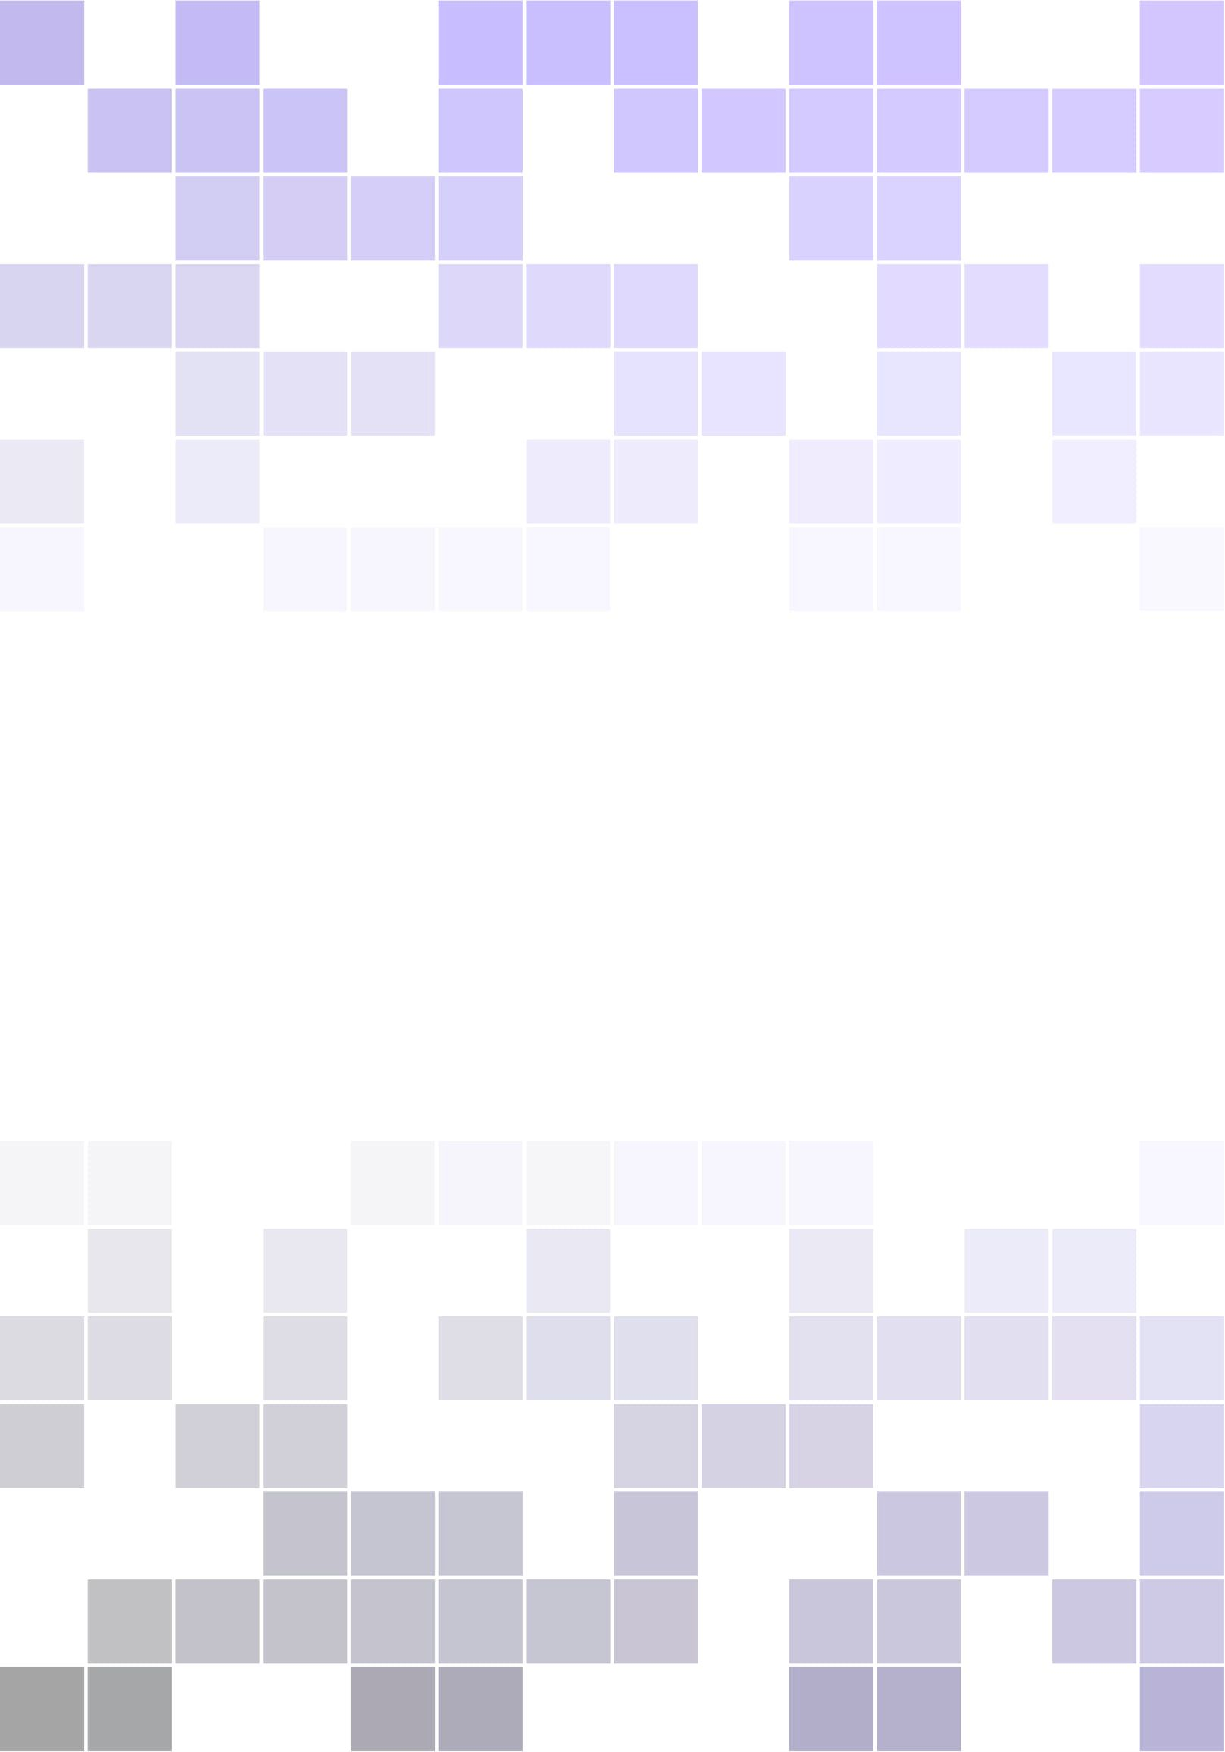
\includegraphics[width=\paperwidth]{background.pdf}};
\draw (current page.center) node [fill=ocre!30!white,fill opacity=0.6,text opacity=1,inner sep=1cm]{\Huge\centering\bfseries\parbox[c][][t]{\paperwidth}{\centering\rl{ 
			پیشنهادنامه‌ی سامانه‌ی برخط تسهیم هزینه‌ها با دوستان}
			\\[15pt] % Book title
{
	\Large
	\rl{
	 تحلیل و طراحی سیستم‌ها
	}
}\\[20pt] % Subtitle
{\huge 
	\rl{
		سامانه‌ی دُنگ
}
}}}; % Author name
\end{tikzpicture}
\vfill
\endgroup

%----------------------------------------------------------------------------------------
%	COPYRIGHT PAGE
%----------------------------------------------------------------------------------------

\newpage
~\vfill
\thispagestyle{empty}

%\noindent Copyright \copyright\ 2019 John Smith\\ % Copyright notice
%
%\noindent \textsc{Published by Publisher}\\ % Publisher
%
%\noindent \textsc{book-website.com}\\ % URL
%
%\noindent Licensed under the Creative Commons Attribution-NonCommercial 3.0 Unported License (the ``License''). You may not use this file except in compliance with the License. You may obtain a copy of the License at \url{http://creativecommons.org/licenses/by-nc/3.0}. Unless required by applicable law or agreed to in writing, software distributed under the License is distributed on an \textsc{``as is'' basis, without warranties or conditions of any kind}, either express or implied. See the License for the specific language governing permissions and limitations under the License.\\ % License information, replace this with your own license (if any)
%\noindent \textit{First printing, March 2019} % Printing/edition date

\begin{tabular}{rl}
	حمیدرضا هدایتی	&	
	۹۶۱۰۹۹۳۹
	\\
	ایمان غلامی &
	۹۶۱۰۹۸۰۹\\
	آرمین سعادت &
	۹۶۱۰۵۸۲۹
\end{tabular}\\\\

\noindent\textbf{کارفرما}:
آزمایشگاه مهندسی خودکار نرم‌افزار - دانشگاه صنعتی شریف


%----------------------------------------------------------------------------------------
%	TABLE OF CONTENTS
%----------------------------------------------------------------------------------------

%\usechapterimagefalse % If you don't want to include a chapter image, use this to toggle images off - it can be enabled later with \usechapterimagetrue

\chapterimage{chapter_head_1.pdf} % Table of contents heading image

\pagestyle{empty} % Disable headers and footers for the following pages

\tableofcontents % Print the table of contents itself

%\cleardoublepage % Forces the first chapter to start on an odd page so it's on the right side of the book

\renewcommand{\arraystretch}{1.7}


\part{
	\rl{
		معرفی پروژه
	}
}


\pagestyle{fancy} 


%----------------------------------------------------------------------------------------
%	PART
%----------------------------------------------------------------------------------------

\chapter{
اهداف
}

%----------------------------------------------------------------------------------------
%	CHAPTER 1
%----------------------------------------------------------------------------------------

%\chapterimage{chapter_head_2.pdf} % Chapter heading image

\section{مقدمه}

یکی از مشکلاتی که دانشجویان دانشگاه صنعتی شریف -  که می‌توان گفت یکی از بهترین دانشگاه‌های ایران است - پس از فارغ‌التحصیلی و یا در حین دانشگاه با آن روبه‌رو هستند یافتن شغل مناسب است.
از طرفی بسیاری از کارفرماها هم در جست‌وجوی نیروی کار متخصص هستند یا می‌خواهند با استخدام نیروهایشان از یک دانشگاه خوب،
جوی نسبتا همگن در شرکت یا سازمانشان ایجاد کنند.

هدف اصلی این پروژه استفاده از فناوری اطلاعات برای تسهیل در دستیابی به این مهم است؛ به گونه‌ای که کارفرماها بتوانند آگهی‌های خود برای موقعیت‌های شغلی موجود در سازمانشان را در آن قرار دهند و دانشجویان بتوانند با مشاهده‌ی این آگهی‌ها، برای موقعیت شغلی مورد نظرشان درخواست بدهند.

البته می‌دانیم برای کاریابی خدمات مشابه زیادی وجود دارد، ولی با توجه به کلی بودن و خاص‌منظوره نبودن آن‌ها، کارآمدی‌ای که یک سامانه‌ی خاص‌منظوره می‌تواند داشته‌باشد را ندارند و دانشجویان شریف رغبت چندانی به استفاده از آن‌ها ندارند و می‌بینیم که به طور معمول برای پیدا کردن فرصت‌های کارآموزی و یا شغل مورد نظرشان به طور مستقیم و یا نهایتا با تبلیغات پوستری آن‌ها در سطح دانشگاه پیدا می‌کنند. اینجاست که نیاز به یک سامانه‌ی اختصاصی برای دانشجویان دانشگاه شریف حس می‌شود و هدف اصلی ما هم این است که این خلا را پر کنیم.

\section{اهداف}

سامانه‌ی شریف‌کار با هدف آسان‌نمودن روند‌های یافتن فرصت‌های کارآموزی، کاریابی، و استخدام نیروی متخصص طراحی شده‌است.
این سامانه خدمات گوناگونی را در راستای رفع نیازهای دانشجویان، فارغ‌التحصیلان و خود عرضه می‌کند.
ثبت آگهی‌های شغلی، امکان جستجوی کار، کارفرما و دانشجویان براساس، امکان استخدام دانشجویان و ... .
تا در نهایت هم دانشجویان بتوانند سریع‌تر و ساده‌تر فرصت‌های شغلی مورد نظرشان را پیدا کنند و هم کافرماها بتوانند سریع‌تر و ساده‌تر و کم‌هزینه‌تر به نیروی متخصص مورد نیازشان دست‌یابند.

%\section{Paragraphs of Text}\index{Paragraphs of Text}
%
%\lipsum[1-7] % Dummy text
%
%%------------------------------------------------
%
%\section{Citation}\index{Citation}
%
%This statement requires citation \cite{article_key}; this one is more specific \cite[162]{book_key}.
%
%%------------------------------------------------
%
%\section{Lists}\index{Lists}
%
%Lists are useful to present information in a concise and/or ordered way\footnote{Footnote example...}.
%
%\subsection{Numbered List}\index{Lists!Numbered List}
%
%\begin{enumerate}
%	\item The first item
%	\item The second item
%	\item The third item
%\end{enumerate}
%
%\subsection{Bullet Points}\index{Lists!Bullet Points}
%
%\begin{itemize}
%	\item The first item
%	\item The second item
%	\item The third item
%\end{itemize}
%
%\subsection{Descriptions and Definitions}\index{Lists!Descriptions and Definitions}
%
%\begin{description}
%	\item[Name] Description
%	\item[Word] Definition
%	\item[Comment] Elaboration
%\end{description}
%
%%----------------------------------------------------------------------------------------
%%	CHAPTER 2
%%----------------------------------------------------------------------------------------
%
%\chapter{In-text Elements}
%
%\section{Theorems}\index{Theorems}
%
%This is an example of theorems.
%
%\subsection{Several equations}\index{Theorems!Several Equations}
%This is a theorem consisting of several equations.
%
%\begin{theorem}[Name of the theorem]
%	In $E=\mathbb{R}^n$ all norms are equivalent. It has the properties:
%	\begin{align}
%	& \big| ||\mathbf{x}|| - ||\mathbf{y}|| \big|\leq || \mathbf{x}- \mathbf{y}||\\
%	&  ||\sum_{i=1}^n\mathbf{x}_i||\leq \sum_{i=1}^n||\mathbf{x}_i||\quad\text{where $n$ is a finite integer}
%	\end{align}
%\end{theorem}
%
%\subsection{Single Line}\index{Theorems!Single Line}
%This is a theorem consisting of just one line.
%
%\begin{theorem}
%	A set $\mathcal{D}(G)$ in dense in $L^2(G)$, $|\cdot|_0$. 
%\end{theorem}
%
%%------------------------------------------------
%
%\section{Definitions}\index{Definitions}
%
%This is an example of a definition. A definition could be mathematical or it could define a concept.
%
%\begin{definition}[Definition name]
%	Given a vector space $E$, a norm on $E$ is an application, denoted $||\cdot||$, $E$ in $\mathbb{R}^+=[0,+\infty[$ such that:
%	\begin{align}
%	& ||\mathbf{x}||=0\ \Rightarrow\ \mathbf{x}=\mathbf{0}\\
%	& ||\lambda \mathbf{x}||=|\lambda|\cdot ||\mathbf{x}||\\
%	& ||\mathbf{x}+\mathbf{y}||\leq ||\mathbf{x}||+||\mathbf{y}||
%	\end{align}
%\end{definition}
%
%%------------------------------------------------
%
%\section{Notations}\index{Notations}
%
%\begin{notation}
%	Given an open subset $G$ of $\mathbb{R}^n$, the set of functions $\varphi$ are:
%	\begin{enumerate}
%		\item Bounded support $G$;
%		\item Infinitely differentiable;
%	\end{enumerate}
%	a vector space is denoted by $\mathcal{D}(G)$. 
%\end{notation}
%
%%------------------------------------------------
%
%\section{Remarks}\index{Remarks}
%
%This is an example of a remark.
%
%\begin{remark}
%	The concepts presented here are now in conventional employment in mathematics. Vector spaces are taken over the field $\mathbb{K}=\mathbb{R}$, however, established properties are easily extended to $\mathbb{K}=\mathbb{C}$.
%\end{remark}
%
%%------------------------------------------------
%
%\section{Corollaries}\index{Corollaries}
%
%This is an example of a corollary.
%
%\begin{corollary}[Corollary name]
%	The concepts presented here are now in conventional employment in mathematics. Vector spaces are taken over the field $\mathbb{K}=\mathbb{R}$, however, established properties are easily extended to $\mathbb{K}=\mathbb{C}$.
%\end{corollary}
%
%%------------------------------------------------
%
%\section{Propositions}\index{Propositions}
%
%This is an example of propositions.
%
%\subsection{Several equations}\index{Propositions!Several Equations}
%
%\begin{proposition}[Proposition name]
%	It has the properties:
%	\begin{align}
%	& \big| ||\mathbf{x}|| - ||\mathbf{y}|| \big|\leq || \mathbf{x}- \mathbf{y}||\\
%	&  ||\sum_{i=1}^n\mathbf{x}_i||\leq \sum_{i=1}^n||\mathbf{x}_i||\quad\text{where $n$ is a finite integer}
%	\end{align}
%\end{proposition}
%
%\subsection{Single Line}\index{Propositions!Single Line}
%
%\begin{proposition} 
%	Let $f,g\in L^2(G)$; if $\forall \varphi\in\mathcal{D}(G)$, $(f,\varphi)_0=(g,\varphi)_0$ then $f = g$. 
%\end{proposition}
%
%%------------------------------------------------
%
%\section{Examples}\index{Examples}
%
%This is an example of examples.
%
%\subsection{Equation and Text}\index{Examples!Equation and Text}
%
%\begin{example}
%	Let $G=\{x\in\mathbb{R}^2:|x|<3\}$ and denoted by: $x^0=(1,1)$; consider the function:
%	\begin{equation}
%	f(x)=\left\{\begin{aligned} & \mathrm{e}^{|x|} & & \text{si $|x-x^0|\leq 1/2$}\\
%	& 0 & & \text{si $|x-x^0|> 1/2$}\end{aligned}\right.
%	\end{equation}
%	The function $f$ has bounded support, we can take $A=\{x\in\mathbb{R}^2:|x-x^0|\leq 1/2+\epsilon\}$ for all $\epsilon\in\intoo{0}{5/2-\sqrt{2}}$.
%\end{example}
%
%\subsection{Paragraph of Text}\index{Examples!Paragraph of Text}
%
%\begin{example}[Example name]
%	\lipsum[2]
%\end{example}
%
%%------------------------------------------------
%
%\section{Exercises}\index{Exercises}
%
%This is an example of an exercise.
%
%\begin{exercise}
%	This is a good place to ask a question to test learning progress or further cement ideas into students' minds.
%\end{exercise}
%
%%------------------------------------------------
%
%\section{Problems}\index{Problems}
%
%\begin{problem}
%	What is the average airspeed velocity of an unladen swallow?
%\end{problem}
%
%%------------------------------------------------
%
%\section{Vocabulary}\index{Vocabulary}
%
%Define a word to improve a students' vocabulary.
%
%\begin{vocabulary}[Word]
%	Definition of word.
%\end{vocabulary}


%----------------------------------------------------------------------------------------
%	PART
%----------------------------------------------------------------------------------------


\chapter{
	پیش‌زمینه‌ی پروژه
}

%----------------------------------------------------------------------------------------
%	CHAPTER 2
%----------------------------------------------------------------------------------------

%\chapterimage{chapter_head_2.pdf} % Chapter heading image

\section{طرح مسئله}
سامانه‌های بهبود زندگی روزمره افراد در راستای صرفه‌جویی در یکی از موارد وقت، پول و انرژی بوجود آمده‌اند، سامانه دُنگ تلاش کرده که با تمرکز با  حداقل کردن هزینه زمانی کاربران و همچنین کمینه کردن گردش پول اضافه دو مورد اول را تا حد ممکن کاهش دهد و همچنین با ساده طراحی شدن حداکثری سامانه انرژی بسیار اندکی از کاربران برای ثبت اطلاعات بگیرد که بتواند در ماموریت خود موفق باشد. 

مشکلی که دُنگ در راستای حل آن کوشش می‌کند ایجاد رویکردی منصفانه در گروه‌های دوستی، کاری و خانواده است به صورتی که افراد از بودن کنار یک‌دیگر لذت ببرند و تا حد ممکن درگیر فرآیند‌های خشکی مانند پرداخت بدهی و ... نشوند.


\section{پیشینه‌ی منجرشونده به تعریف پروژه}% \lr{History leading to project request}} :-????????

یکی از بزرگ‌ترین چالش‌های گروه‌های مختلف دوستی و کاری در سرتاسر جهان مفهوم تسهیم هزینه‌ها با دوستان است، زیرا اغلب اوقات در یک گروه خاص فردی «مادر خرج» می‌شود و پس از آن دوستانش به سهو (یا حتی عمد!) فراموش می‌کنند که سهم خود را پرداخت کنند یا حتی آمار حساب پرداختی‌ها و بدهی‌ها را از دست می‌دهند.

تا کنون این مشکل با استفاده از روش‌های سنتی مانند نوشتن یا ذخیره کردن خرج‌ها و محاسبه دستی و زمان‌گیر میزان جابجایی‌های که لازم است انجام بگیرد، حل می‌شده که تمامی این راه‌حل‌ها بسیار زمان‌گیر و انرژی‌بر است و معمولا افراد حاضر نمی‌شوند که چنین هزینه‌ای را بدهند و چنین مسائل مالی خشک و ناراحت‌کننده‌ای را وارد فضاهای دوستی و خانوادگی خود بکنند.

از طرفی جز از سمت افرادی که معمولا پرداخت‌ها را انجام می‌دهند، برای افرادی که قرضی گرفته‌اند یا خرجی برایشان انجام شده هم سخت است که لیست تمامی پول‌هایی که باید در آینده پرداخت کنند را نگه‌ دارند، لذا در این بخش از محیط دوستانه و خرج‌ها هم خلاءی حس می‌شود که لازم است راه‌حلی ارائه شود که مشکل برطرف گردد.

از سویی دیگر هم گاهی اوقات دایره پرداختی‌ها آنقدر پیچیده می‌شود که میزان پول خرد و کارمزد بانک‌ها باعث می‌شود به طور کلی انتقال پول‌ها به صرفه در نظر نرسد، در حالی که می‌توانستیم با کمینه کردن تراکنش‌ها و تغییر شروع و مبدا پرداختی‌ها این میزان را کمتر کنیم و دغدغه کاربران را کاهش دهیم.

تمامی موارد بالا باعث شده‌اند که سامانه دُنگ بوجود بیاید، این سامانه به کاربران که گستره آن ها تمامی افراد جامعه هستند کمک می‌کند تا وضعیت مالی خود و روابط دوستانه خود را بهبود ببخشند.


\section{اهداف}
هدف اصلی این پروژه، طراحی، پیاده‌سازی و اجرای یک سامانه‌ی برخط است که کاربران مختلف به‌کمک آن بتوانند خرج‌های انجام شده را ثبت کرده و افراد مرتبط به آن‌ خرج‌ها را از میان دوستان خود در سامانه انتخاب کنند. این سامانه ویژگی‌های مختلفی را پوشش می‌دهد که از خرج‌های گروهی تا خرج‌های فرد به فرد را شامل می‌شود.

پس به طور کلی و خلاصه، این سامانه تلاش می‌کند تا اهداف زیر را برآورده سازد:
\begin{itemize}
	\item
	سامانه‌ای برای وارد کردن خرج‌های انجام شده با جزییات آن خرج‌ها و افراد درگیر آن باشد.
	\item 
	سامانه‌ای باشد که در صورت اقدام کاربر به اطلاع پیدا کردن از بدهی‌ها و قرض‌هایی که داده بتواند اطلاعات را به آن فرد ارائه کند.
	\item 
	بستری باشد که کاربران بتوانند با ایجاد گروه‌ها به سادگی به خرج‌های جمعی رسیدگی کنند.
	\item
	بتواند با انجام بهینه‌سازی تعداد گردش پول‌ها و پول‌های خرد را کمتر کند.
\end{itemize}

\section{توصیف محصول}
محصول نهایی، سامانه دُنگ خواهد بود. همانطور که پیش‌تر هم اشاره کردیم، هدف نهایی این سامانه بهبود زندگی روزمره کاربران است.

در این سامانه تنها یک دسته کاربر عمومی وجود دارد، که پس از ایجاد حساب کاربری، وارد حساب کاربری خود شده و می‌تواند هزینه‌ها را به صورت گروهی (توانایی ساختن گروه با دوستان و همچنین اضافه کردن دوست به حساب کاربری وجود دارد) یا تکی وارد کند. حساب‌کاربری با ایمیل و شماره تلفن و هزینه‌ها با تاریخ و افراد مرتبط و عکس و موقعیت مکانی مشخص می‌شوند و کاربران می توانند با استفاده از ایمیل یا شماره تلفن فردی را به عنوان دوست خود اضافه کنند.

برای سادگی و کمتر کردن هزینه زمانی کاربران، ویژگی هزینه‌های گروهی نیز وجود دارد که می‌توان به صورت دقیق مشخص کرد که هر فرد چه درصدی از هزینه کلی را باید پرداخت کند یا اینکه باید هزینه به صورت مساوی میان همه تقسیم شود. همچنین تمامی کاربران می‌توانند با مراجعه به گزارش‌ها بدهی و قرض‌های کنونی و گذشته خود را مشاهده کنند و در صورت توان بدهی‌های خود را پرداخت کنند.

از طرفی سامانه برای کمتر کردن تعداد گردش‌های پولی، در صورتی که می‌توان با جابجایی پرداخت‌ها و حذف افراد میانی تعداد گردش پول‌ها را کمتر کرد در گروه‌های تشکیل شده بهینه‌سازی برای پرداخت‌ها انجام می‌دهد.




%\section{Paragraphs of Text}\index{Paragraphs of Text}
%
%\lipsum[1-7] % Dummy text
%
%%------------------------------------------------
%
%\section{Citation}\index{Citation}
%
%This statement requires citation \cite{article_key}; this one is more specific \cite[162]{book_key}.
%
%%------------------------------------------------
%
%\section{Lists}\index{Lists}
%
%Lists are useful to present information in a concise and/or ordered way\footnote{Footnote example...}.
%
%\subsection{Numbered List}\index{Lists!Numbered List}
%
%\begin{enumerate}
%	\item The first item
%	\item The second item
%	\item The third item
%\end{enumerate}
%
%\subsection{Bullet Points}\index{Lists!Bullet Points}
%
%\begin{itemize}
%	\item The first item
%	\item The second item
%	\item The third item
%\end{itemize}
%
%\subsection{Descriptions and Definitions}\index{Lists!Descriptions and Definitions}
%
%\begin{description}
%	\item[Name] Description
%	\item[Word] Definition
%	\item[Comment] Elaboration
%\end{description}
%
%%----------------------------------------------------------------------------------------
%%	CHAPTER 2
%%----------------------------------------------------------------------------------------
%
%\chapter{In-text Elements}
%
%\section{Theorems}\index{Theorems}
%
%This is an example of theorems.
%
%\subsection{Several equations}\index{Theorems!Several Equations}
%This is a theorem consisting of several equations.
%
%\begin{theorem}[Name of the theorem]
%	In $E=\mathbb{R}^n$ all norms are equivalent. It has the properties:
%	\begin{align}
%	& \big| ||\mathbf{x}|| - ||\mathbf{y}|| \big|\leq || \mathbf{x}- \mathbf{y}||\\
%	&  ||\sum_{i=1}^n\mathbf{x}_i||\leq \sum_{i=1}^n||\mathbf{x}_i||\quad\text{where $n$ is a finite integer}
%	\end{align}
%\end{theorem}
%
%\subsection{Single Line}\index{Theorems!Single Line}
%This is a theorem consisting of just one line.
%
%\begin{theorem}
%	A set $\mathcal{D}(G)$ in dense in $L^2(G)$, $|\cdot|_0$. 
%\end{theorem}
%
%%------------------------------------------------
%
%\section{Definitions}\index{Definitions}
%
%This is an example of a definition. A definition could be mathematical or it could define a concept.
%
%\begin{definition}[Definition name]
%	Given a vector space $E$, a norm on $E$ is an application, denoted $||\cdot||$, $E$ in $\mathbb{R}^+=[0,+\infty[$ such that:
%	\begin{align}
%	& ||\mathbf{x}||=0\ \Rightarrow\ \mathbf{x}=\mathbf{0}\\
%	& ||\lambda \mathbf{x}||=|\lambda|\cdot ||\mathbf{x}||\\
%	& ||\mathbf{x}+\mathbf{y}||\leq ||\mathbf{x}||+||\mathbf{y}||
%	\end{align}
%\end{definition}
%
%%------------------------------------------------
%
%\section{Notations}\index{Notations}
%
%\begin{notation}
%	Given an open subset $G$ of $\mathbb{R}^n$, the set of functions $\varphi$ are:
%	\begin{enumerate}
%		\item Bounded support $G$;
%		\item Infinitely differentiable;
%	\end{enumerate}
%	a vector space is denoted by $\mathcal{D}(G)$. 
%\end{notation}
%
%%------------------------------------------------
%
%\section{Remarks}\index{Remarks}
%
%This is an example of a remark.
%
%\begin{remark}
%	The concepts presented here are now in conventional employment in mathematics. Vector spaces are taken over the field $\mathbb{K}=\mathbb{R}$, however, established properties are easily extended to $\mathbb{K}=\mathbb{C}$.
%\end{remark}
%
%%------------------------------------------------
%
%\section{Corollaries}\index{Corollaries}
%
%This is an example of a corollary.
%
%\begin{corollary}[Corollary name]
%	The concepts presented here are now in conventional employment in mathematics. Vector spaces are taken over the field $\mathbb{K}=\mathbb{R}$, however, established properties are easily extended to $\mathbb{K}=\mathbb{C}$.
%\end{corollary}
%
%%------------------------------------------------
%
%\section{Propositions}\index{Propositions}
%
%This is an example of propositions.
%
%\subsection{Several equations}\index{Propositions!Several Equations}
%
%\begin{proposition}[Proposition name]
%	It has the properties:
%	\begin{align}
%	& \big| ||\mathbf{x}|| - ||\mathbf{y}|| \big|\leq || \mathbf{x}- \mathbf{y}||\\
%	&  ||\sum_{i=1}^n\mathbf{x}_i||\leq \sum_{i=1}^n||\mathbf{x}_i||\quad\text{where $n$ is a finite integer}
%	\end{align}
%\end{proposition}
%
%\subsection{Single Line}\index{Propositions!Single Line}
%
%\begin{proposition} 
%	Let $f,g\in L^2(G)$; if $\forall \varphi\in\mathcal{D}(G)$, $(f,\varphi)_0=(g,\varphi)_0$ then $f = g$. 
%\end{proposition}
%
%%------------------------------------------------
%
%\section{Examples}\index{Examples}
%
%This is an example of examples.
%
%\subsection{Equation and Text}\index{Examples!Equation and Text}
%
%\begin{example}
%	Let $G=\{x\in\mathbb{R}^2:|x|<3\}$ and denoted by: $x^0=(1,1)$; consider the function:
%	\begin{equation}
%	f(x)=\left\{\begin{aligned} & \mathrm{e}^{|x|} & & \text{si $|x-x^0|\leq 1/2$}\\
%	& 0 & & \text{si $|x-x^0|> 1/2$}\end{aligned}\right.
%	\end{equation}
%	The function $f$ has bounded support, we can take $A=\{x\in\mathbb{R}^2:|x-x^0|\leq 1/2+\epsilon\}$ for all $\epsilon\in\intoo{0}{5/2-\sqrt{2}}$.
%\end{example}
%
%\subsection{Paragraph of Text}\index{Examples!Paragraph of Text}
%
%\begin{example}[Example name]
%	\lipsum[2]
%\end{example}
%
%%------------------------------------------------
%
%\section{Exercises}\index{Exercises}
%
%This is an example of an exercise.
%
%\begin{exercise}
%	This is a good place to ask a question to test learning progress or further cement ideas into students' minds.
%\end{exercise}
%
%%------------------------------------------------
%
%\section{Problems}\index{Problems}
%
%\begin{problem}
%	What is the average airspeed velocity of an unladen swallow?
%\end{problem}
%
%%------------------------------------------------
%
%\section{Vocabulary}\index{Vocabulary}
%
%Define a word to improve a students' vocabulary.
%
%\begin{vocabulary}[Word]
%	Definition of word.
%\end{vocabulary}


\makeatletter
\def\titlefootnote{\ifx\protect\@typeset@protect\expandafter\LTRfootnote\else\expandafter\@gobble\fi}
\makeatother

\chapter{گستره}
	\section{ذینفع‌های سامانه \titlefootnote{Stakeholders}
	}
	\subsection{مالکین}
	مالک این سامانه دکتر حیدرنوری استاد درس تحلیل و طراحی سیستم‌ها است. انتظار ایشان از این سامانه عملیاتی شدن سامانه برای ارائه به کاربران در صورت وجود زیرساخت‌های مناسب و برآورده شدن حداقل‌های مالی است.
	
	\subsection{کاربران}
کاربران این سامانه دو دسته هستند:
\begin{enumerate}
\item \textbf{کاربران عمومی:}
	کاربرانی هستند که با ثبت‌نام در سامانه و تکمیل کردن حساب کاربری خود به دنبال اضافه کردن دوست در  سامانه و ایجاد گروه‌ها هستند که خرج‌ها را وارد کرده و بدهی‌ها را پرداخت کنند.

\item \textbf{مدیران سامانه:}
مدیران سامانه با دسترسی به اطلاعات تمامی کاربران و گروه‌ها توانایی مشاهده تمامی گزارشات مالی سامانه را دارند.
\end{enumerate}

\subsection{تحلیلگران، طراح‌ها و سازندگان سامانه}

تیم ۳ نفره‌ی معرفی شده در آغاز پیشنهادنامه به شکل گروهی هر سه وظیفه‌ی تحلیل، طراحی و توسعه‌ی سامانه را بر عهده دارد.

\subsection{مدیر پروژه}

\subsection{فراهم کنندگان زیرساخت‌های سرویس و سرویس‌های خارجی}
از 
\lr{Google Maps} 
برای نشان دادن موقعیت جغرافیایی موقعییت‌های شغلی در نقشه استفاده می‌شود همچنین از زیرساخت ابری \lr{ArvanCloud} برای نگه‌داری و ذخیره‌سازی اطلاعات بر روی فضای ابری استفاده خواهد شد، همچنین برای سرویس \lr{CI/CD} از سرویس \lr{Github} استفاده می‌شود.

\section{داده‌ها}
داده‌هایی که توسط این سیستم مدیریت می‌شوند موارد زیر هستند:
\begin{enumerate}
\item \textbf{اطلاعات کاربران:}
هر کاربر این سامانه یک حساب کاربری دارد. این حساب کاربری شامل ایمیل و شماره تلفن می‌شود که هنگام ثبت‌نام کاربر از او گرفته می‌شود. هر کاربر علاوه بر اطلاعات شخصی خود تعدادی دوست در سامانه دارد که می‌تواند با آن‌ها خرج رد و بدل کند. هر کاربر علاوه بر حساب کاربری میزان بدهی کلی و میزان طلب کلی‌ا‌ش مشخص شده است.
\item \textbf{گروه‌ها:}
گروه‌ها تعدادی از کاربران هستند که توسط یک نفر تشکیل می‌شوند. به ازای هر گروه اطلاعاتی مانند خرج‌های آن گروه ذخیره شده است.
\item \textbf{خرج‌ها:}
هر خرج یک کاربر به عنوان خرج کننده و یک کاربر یا گروه به عنوان بدهکار دارد، هر خرج اطلاعاتی مانند عکس، موقعیت جغرافیایی، تاریخ و اسم می‌تواند داشته باشد. خرج‌های هر کاربر قابل دسترسی هستند.
\end{enumerate}

\section{امکانات}
\subsection{
امکانات مربوط به کاربران} 
\begin{itemize}
	\item
	امکان ثبت خرج برای تک نفر
	\item
	امکان ثبت خرج برای یک گروه به صورت مساوی
	\item
	امکان ثبت خرج برای یک گروه به صورت وزن‌دار
	\item
	امکان مشاهده تاریخه بدهی‌ها و طلب‌ها
	 \item
	امکان اضافه کردن یک دوست 
		 \item
	امکان ساخت گروه با دوستان
		 \item
	امکان پرداخت یک بدهی 
\end{itemize}
\subsection{
امکانات مربوط به مدیران سامانه}
\begin{itemize}
	\item 
امکان ایجاد حساب کاربری (دریافت اطلاعات مورد نیاز از هر فرد) و تایید ثبت‌نام 
\item 
امکان ویرایش حساب‌های کاربری، لیست دوستان هر فرد و افراد گروه‌ها
 \item 
امکان ویرایش خرج‌های فردی و گروهی
\item
امکان مشاهده گزارش‌های مالی هر کاربر
\end{itemize}

\section{گستردگی مکانی}
با توجه به اینکه نسخه اولیه قابل ارائه سرویس به زبان فارسی ارائه می‌شود تمامی فارسی زبانان می‌توانند از این سرویس استفاده کنند.


\part{
	\rl{
		مسیر و مدیریت پروژه
	}
}


%----------------------------------------------------------------------------------------
%	PART
%----------------------------------------------------------------------------------------


\chapter{
	رویکرد پروژه 
}

%----------------------------------------------------------------------------------------
%	CHAPTER 4
%----------------------------------------------------------------------------------------

%\chapterimage{chapter_head_2.pdf} % Chapter heading image
رویکرد پروژه به‌صورت محصول‌محور
\LTRfootnote{Product driven}
خواهد بود. محصول‌محور در مقابل مشتری‌محور 
\LTRfootnote{Customer driven}
مطرح می‌شود و به این معناست که ابتدا محصول طراحی و تولید شده سپس به مسائل مربوط به جذب مشتری، تحلیل متقاضیان و خواسته‌های آن‌ها، جستجوی بازار مناسب و دیگر مسائل مربوط به این دسته پرداخته می‌شود. در حالی که در رویکرد مشتری‌محور ایتدا بازار هدف به صورت دقیق مشخص و شناسایی می‌شود و با مشتریان تعامل صورت می‌گیرد. در این تعاملات، خواسته‌ها و نیازهای مشتریان مشخص شده و محصول مورد نظر برای رفع نیازهای مطرح شده مطرح می‌شود.
رویکرد محصول‌محور ریسک بیشتری دارد چرا که بر این فرض استوار است که محصول نهایی یک حفره را پر خواهد کرد و بازار مناسبی خواهد داشت.

از روش توسعه‌ی چابک نرم‌افزار 
\LTRfootnote{Agile software development}
به عنوان فرایند پیشبرد پروژه استفاده خواهیم کرد. 
این روش مبتنی بر تکرار است. این روش برنامه‌ریزی تطبیقی، توسعه و تحویل تکاملی و رویکرد زمان بسته‌بندی تکرارشونده را ارتقا می‌بخشد و پاسخ‌های سریع و انعطاف‌پذیر برای انجام تغییرات را تقویت می‌کند. این یک روش تدریجی می‌باشد که در آن از حجم طراحی‌های کامل مقدم بر اجرا کاسته شده و طراحی  و اجرا و پیاده‌سازی در بسته‌های کوچک با یکدیگر ادغام شده‌اند. 

مسیر پروژه و تحویل‌دادنی‌ها در هر فاز در زیر آمده‌ است.

\begin{figure}[h]
	\centering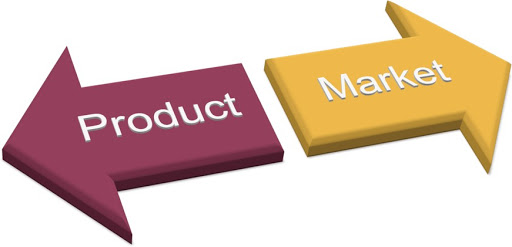
\includegraphics[scale=0.8]{product_vs_customer2}
	\caption{رویکرد پروژه}
	\label{phases} % Unique label used for referencing the figure in-text
	%\addcontentsline{toc}{figure}{Figure \ref{fig:placeholder}} % Uncomment to add the figure to the table of contents
\end{figure}


\section{مسیر پروژه}
پروژه از ۵ فاز کلی تشکیل شده است. ۴ فاز اول مربوط به مراحل تولید بوده و در تلاش برای ایجاد محصول می‌باشد. فاز آخر مربوط به مراحل پس از تولید است و در تلاش برای بهبود محصول موجود می‌باشد.

در فاز اول گستره و مسئله را به‌طور دقیق تعریف می‌کنیم. ایده‌ کلی برای محصول را مطرح کرده و استدلال می‌کنیم که این محصول به چه نیازهایی پاسخ خواهد داد.

در فاز دوم، به تحلیل مسئله 
\LTRfootnote{Problem analysis}
پرداخته و به صورت دقیق حفره‌های موجود را بررسی می‌کنیم. به بررسی نیازمندی‌ها 
\LTRfootnote{Requirement analysis}
می‌پردازیم و مطابق با آن‌ها محصول مورد نظر را به صورت دقیق‌تر طراحی می‌کنیم. در طراحی سیستم این نکته در نظر گرفته می‌شود که رضایت تمام ذی‌نفعان تا جای ممکن تامین شود. بررسی نیازمندی‌ها به جلب رضایت کاربران به عنوان یکی از مهم‌ترین ذی‌نفعان کمک بسیار می‌کند.
در این فاز سناریو‌های سیستم را طراحی می‌کنیم و نمودار مورد کاربرد 
\LTRfootnote{Problem analysis}
را با توجه به نیازمندی‌ها و به روش اصولی به‌دست خواهیم آورد. یعنی ابتدا اکتورها و موردکاربردها و سپس روابط بین آن‌ها را به‌دست خواهیم آورد.

فاز سوم مربوط به مدل‌سازی فرآیندها است. در این مرحله در سطح منطقی 
\LTRfootnote{Logical design}
به طراحی سیستم و فرآیند‌های آن می‌پردازیم، موجودیت‌‌ها را طراحی می‌کنیم، بانک‌های اطلاعاتی را تشکیل می‌دهیم و روابط بین موجودیت‌ها را مشخص می‌کنیم.

فاز چهارم مربوط به پیاده‌سازی و ارزیابی سامانه است. با توجه به طراحی‌ها و مدل‌سازی‌های انجام شده در فازهای قبلی،‌ در قالب فرآیند چابک اسکرام به پیاده‌سازی محصول می‌پردازیم. نکته مهم در این بخش، تداوم و همگامی ارزیابی و پیاده‌سازی است. به این معنا که فرآیند پیاده‌سازی به تعدادی زیربخش تقسیم می‌شود. پس از پایان هر زیربخش، ابتدا عملکرد آن مورد بررسی و ارزیابی دقیق قرار می‌گیرد و در صورت تایید ب مرحله بعدی پیاده‌سازی می‌رویم. این کار در نگاه اول فرآیند پیاده‌سازی را طولانی و زمان‌گیرتر جلوه می‌دهد. اما در نهایت تاثیر به سزایی در بهبود زمان و انرژی مصرف شده خواهد گذاشت. با تقسیم پیاده‌سازی کلی به تعدادی زیربخش، دقت روی هر بخش زیاد شده و ارزیابی دقیقی روی آن صورت می‌گیرد. در این حالت پیدا کردن ایرادات فنی و غیرفنی و برطرف کردن آن‌ها راحت‌تر است. 
نکته دیگر که حائز اهمیت است، تداوم مستندسازی در این فاز است. مستندسازی نیز در نگاه اول به عنوان یک سربار دیده می‌شود اما مستند سازی نقش بسزایی در کاهش هزینه‌های مربوط به نگه‌داری از محصول دارد که در کاهش هزینه‌های نهایی محصول سهم اصلی خواهد داشت.

فاز پنجم مربوط به ارزیابی کلی سامانه به عنوان یک محصول کامل است. حالت کامل این ارزیابی زمانی تحقق می‌یابد که محصول کامل و آماده شده باشد و توسط کاربران (هرچند محدود) استفاده شود.
هدف از این بخش مانیتور کردن عملکرد محصول و اعلام ایرادات احتمالی جهت رفع آن‌ها می‌باشد.

\begin{figure}[h]
	\centering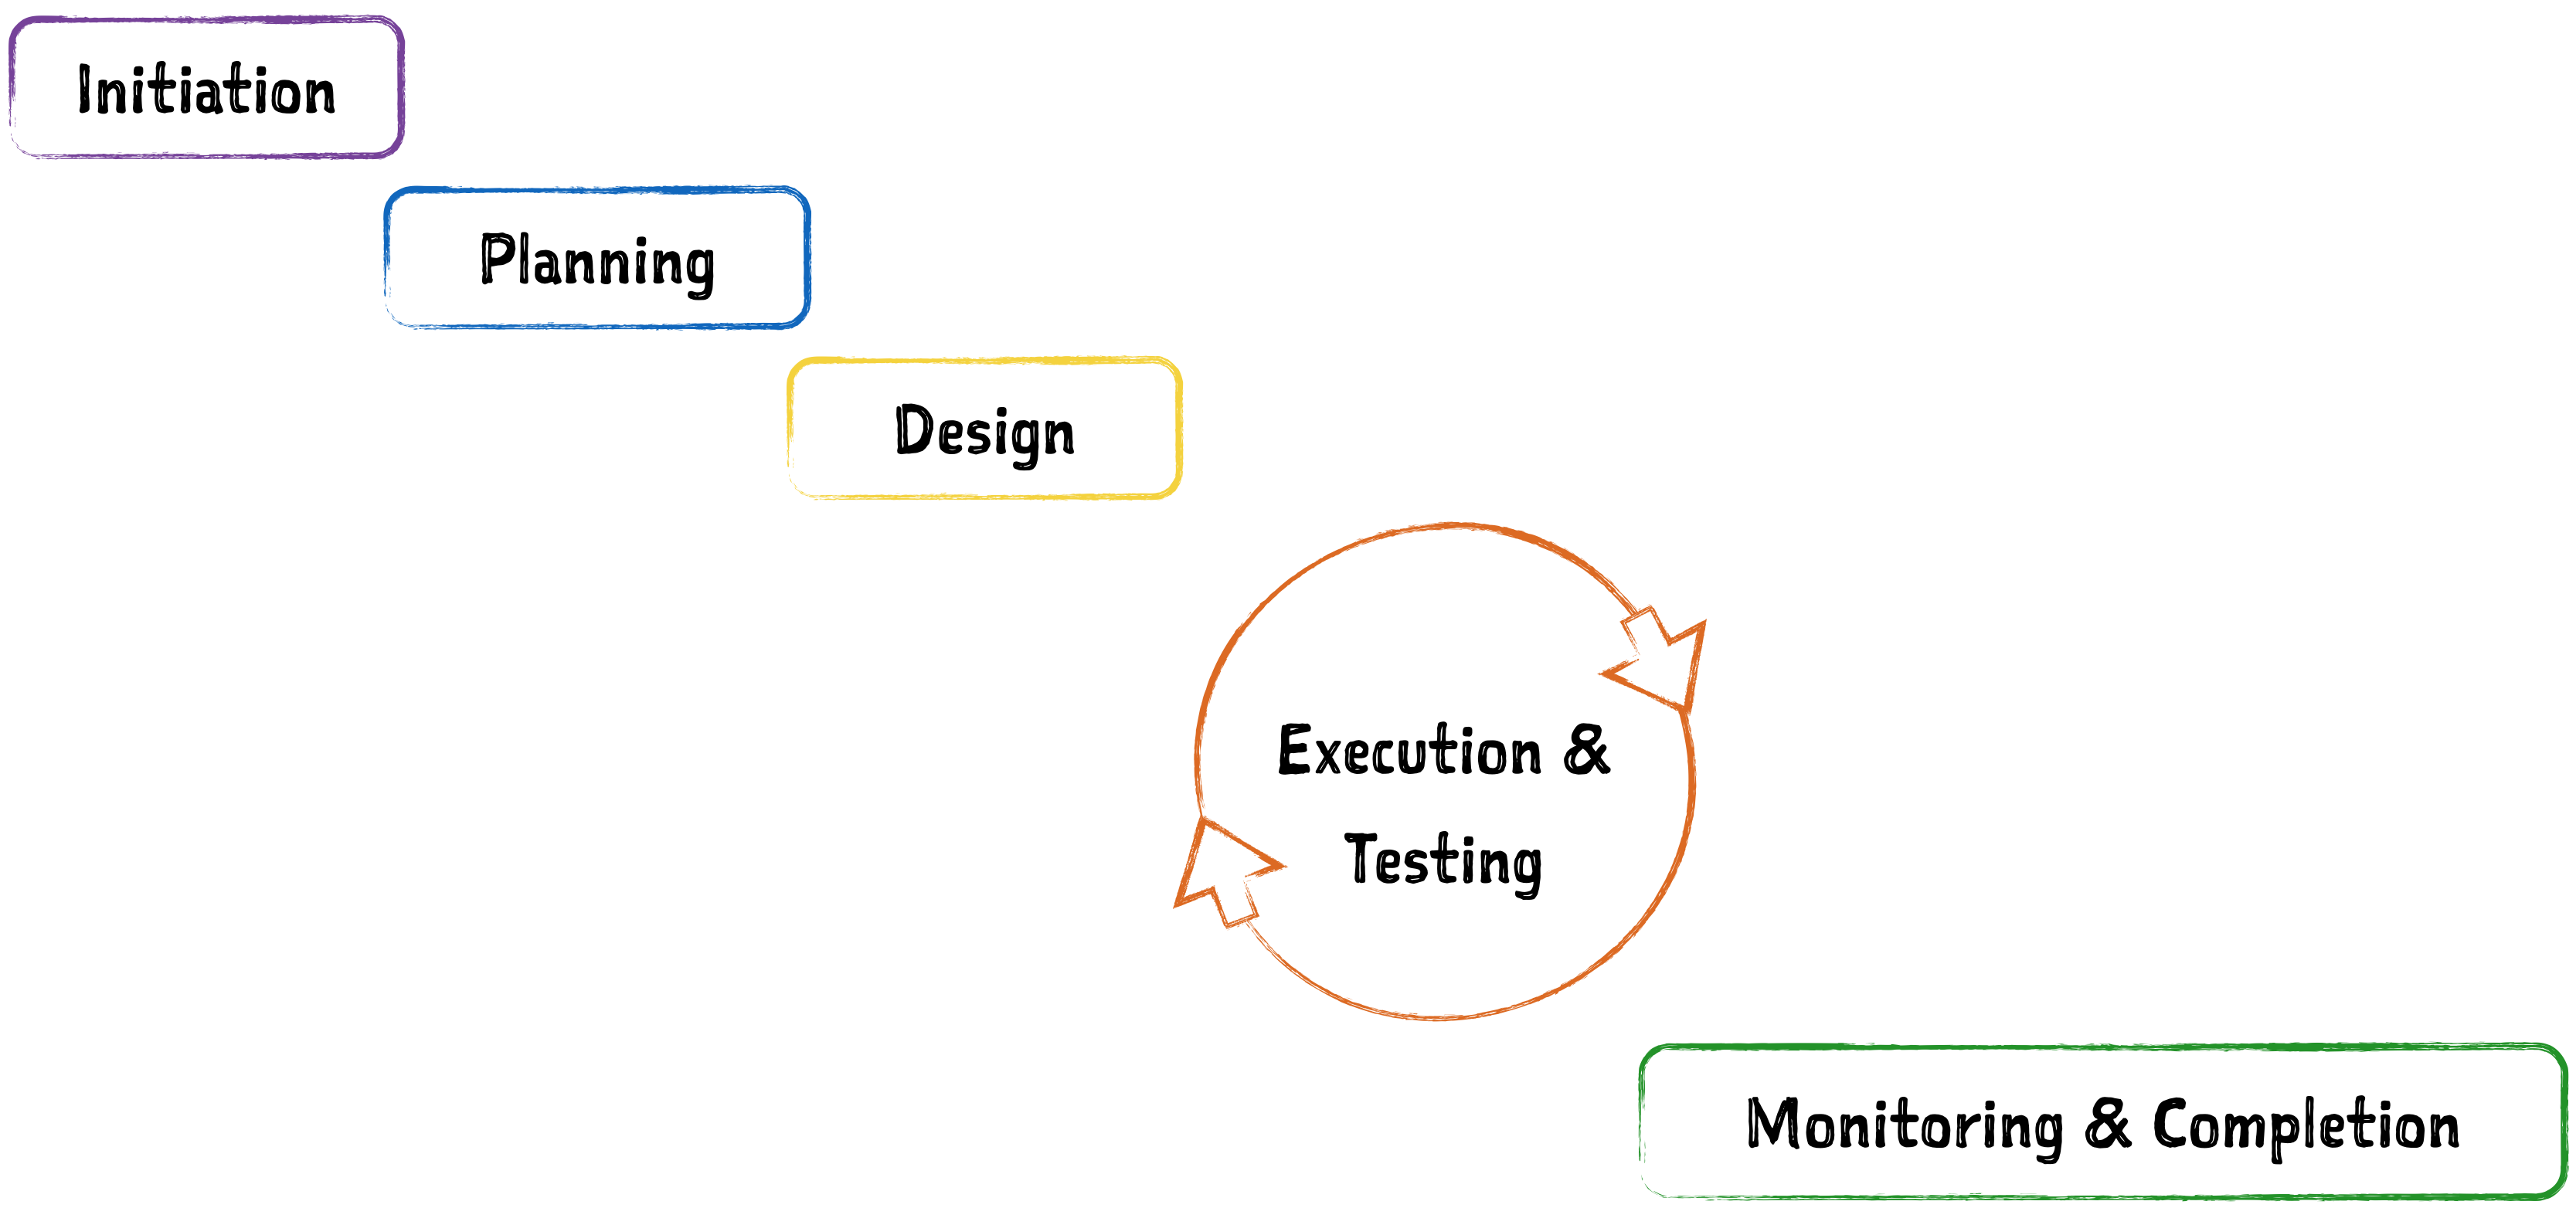
\includegraphics[scale=0.25]{proj_phases}
	\caption{مسیر پروژه}
	\label{phases} % Unique label used for referencing the figure in-text
	%\addcontentsline{toc}{figure}{Figure \ref{fig:placeholder}} % Uncomment to add the figure to the table of contents
\end{figure}

\pagebreak
\section{تحویل‌دادنی‌ها}
تحویل‌دادنی‌های هر فاز از پروژه به‌صورت زیر خواهد بود:

\begin{itemize}
	\item 
	فاز اول
	\subitem
	پیشنهادنامه‌ی پروژه (پروپوزال)
	\subitem نمودار گنت \LTRfootnote{Gantt Chart}
	\subitem نمودار پرت \LTRfootnote{Pert Chart}
	\item 
	فاز دوم
	\subitem  بنمودار مورد استفاده

	
	\item 
	فاز سوم
	\subitem نمودار جریان داده‌ها \LTRfootnote{Data flow Diagram}
	\subitem
	نمودار داده رابطه‌ای
	
	\item 
فاز چهارم
	\subitem نسخه‌ی نهایی «دنگ‌»
	\subitem مستندات پروژه
	
	\item 
	فاز پنجم
	
	\subitem گزارش عملکرد محصول
	\subitem گزارش باگ‌های احتمالی
	\subitem گزارش تغییرات اعمال شده در نسخه‌های جدید
\end{itemize}

\chapter{رهیافت مدیریت}
\section{مدیریت، تجارب و وظایف}
\subsection{مدیر پروژه}
\begin{table}[H]
	\centering
	\resizebox{\textwidth}{!}{%
		\begin{tabular}{|C{0.2\textwidth}C{0.2\textwidth}C{0.2\textwidth}C{0.2\textwidth}C{0.2\textwidth}|}
			\hline
			\rowcolor[HTML]{F36619} 
			\multicolumn{5}{|c|}{\cellcolor[HTML]{008cff}{\color[HTML]{FFFFFF}
					\Large
					\textbf{
						مدیر پروژه
					}
			}}                                   \\ \hline
			\rowcolor[HTML]{c6d8f2} 
			نام و نام خانوادگی
			&               
			مدرک تحصیلی    
			&                
			سابقه‌ی کاری
			&     
			شرح سوابق کاری
			&
			توانمندی‌ها
			\\
			\rowcolor[HTML]{dee5ef} 
			امین رخشا
			&               
			کارشناسی مهندسی کامپیوتر
			&    
			دو ماه
			&              
				کارآموزی در شرکت رهنما،                   
				پروژه‌ی
				buyrapido
			&
			مدیریت پروژه
			\\
			\hline
		\end{tabular}
	}
\end{table}

\subsection{اعضا و سوابق و توانمندی‌ها}
تمامی اعضا در تمامی مراحل از جمله، تحلیل، توسعه و تست نقش خواهند داشت.
\begin{table}[H]
	\centering
	\resizebox{\textwidth}{!}{%
		\begin{tabular}{|C{0.2\textwidth}C{0.2\textwidth}C{0.2\textwidth}C{0.2\textwidth}C{0.2\textwidth}|}
			\hline
			\rowcolor[HTML]{F36619} 
			\multicolumn{5}{|c|}{\cellcolor[HTML]{008cff}{\color[HTML]{FFFFFF}
					\Large
					\textbf{
						اعضا
					}
			}}                                   \\ \hline
			\rowcolor[HTML]{c6d8f2} 
			نام و نام خانوادگی
			&               
			مدرک تحصیلی    
			&                
			سابقه‌ی کاری
			&     
			شرح سوابق کاری
			&
			توانمندی‌ها
			\\
		\rowcolor[HTML]{dee5ef} 
			امین رخشا
			&               
			کارشناسی مهندسی کامپیوتر
			&    
			دو ماه
			&              
			کارآموزی در شرکت رهنما،                   
			پروژه‌ی
			buyrapido
			&
			\lr{Node.js, 
				React Native, Android Programming, CSS, HTML}
			\\
			\rowcolor[HTML]{dee5ef} 
			مهبد مجید
			&               
			کارشناسی مهندسی کامپیوتر
			&    
			دو ماه
			&              
			کارآموزی در شرکت رهنما،                   
			پروژه‌ی
			buyrapido
			&
			\lr{
				MongoDB,
				Node.js, 
				Database Design,
				Backend Development
			}
			\\
			\rowcolor[HTML]{dee5ef} 
			کیمیا حمیدیه
			&               
			کارشناسی مهندسی کامپیوتر
			&    
			دو ماه
			&              
			تیم فنی
			
			\lr{AI Challenge}
			&
			\lr{Django, Docker, Infrastructure, CSS, HTML}
			\\
			\hline
		\end{tabular}
	}
\end{table}

\subsection{تحلیل‌گران}
\begin{table}[H]
	\centering
	\resizebox{\textwidth}{!}{%
		\begin{tabular}{|C{0.25\textwidth}C{0.25\textwidth}C{0.25\textwidth}C{0.25\textwidth}|}
			\hline
			\rowcolor[HTML]{F36619} 
			\multicolumn{4}{|c|}{\cellcolor[HTML]{008cff}{\color[HTML]{FFFFFF}
					\Large
					\textbf{
						تحلیل‌گران
					}
			}}                                   \\ \hline
			\rowcolor[HTML]{c6d8f2} 
			نام و نام خانوادگی
			&               
			مدرک تحصیلی    
			&                
			سابقه‌ی کاری
			&     
			شرح سوابق کاری
			\\
			\rowcolor[HTML]{dee5ef} 
			مهبد مجید
			&               
			کارشناسی مهندسی کامپیوتر
			&    
			دو ماه
			&              
			کارآموزی در شرکت رهنما،                   
			پروژه‌ی
			buyrapido
			\\
			\rowcolor[HTML]{dee5ef} 
			کیمیا حمیدیه
			&               
			کارشناسی مهندسی کامپیوتر
			&    
			دو ماه
			&              
			تیم فنی
			\lr{AI Challenge}
			\\
			\hline
		\end{tabular}
	}
\end{table}

\subsection{طراح پایگاه‌داده}
\begin{table}[H]
	\centering
	\resizebox{\textwidth}{!}{%
		\begin{tabular}{|C{0.25\textwidth}C{0.25\textwidth}C{0.25\textwidth}C{0.25\textwidth}|}
			\hline
			\rowcolor[HTML]{F36619} 
			\multicolumn{4}{|c|}{\cellcolor[HTML]{008cff}{\color[HTML]{FFFFFF}
					\Large
					\textbf{
					طراح پایگاه‌داده
					}
			}}                                   \\ \hline
			\rowcolor[HTML]{c6d8f2} 
			نام و نام خانوادگی
			&               
			مدرک تحصیلی    
			&                
			سابقه‌ی کاری
			&     
			شرح سوابق کاری
			\\
			\rowcolor[HTML]{dee5ef} 
			مهبد مجید
			&               
			کارشناسی مهندسی کامپیوتر
			&    
			دو ماه
			&              
			طراحی پایگاه‌داده و برنامه‌نویسی
			\lr{back-end}
			\\
			\hline
		\end{tabular}
	}
\end{table}


\subsection{طراحی گرافیکی و طراحی صفحات}
\begin{table}[H]
	\centering
	\resizebox{\textwidth}{!}{%
		\begin{tabular}{|C{0.25\textwidth}C{0.25\textwidth}C{0.25\textwidth}C{0.25\textwidth}|}
			\hline
			\rowcolor[HTML]{F36619} 
			\multicolumn{4}{|c|}{\cellcolor[HTML]{008cff}{\color[HTML]{FFFFFF}
					\Large
					\textbf{
						طراحی گرافیکی و طراحی صفحات
					}
			}}                                   \\ \hline
			\rowcolor[HTML]{c6d8f2} 
			نام و نام خانوادگی
			&               
			مدرک تحصیلی    
			&                
			سابقه‌ی کاری
			&     
			شرح سوابق کاری
			\\
			\rowcolor[HTML]{dee5ef} 
			امین رخشا
			&               
			کارشناسی مهندسی کامپیوتر
			&    
			چهار ماه
			&              
			طراحی صفحات وب و برنامه‌نویسی 
			\lr{front-end}
			\\
						\rowcolor[HTML]{dee5ef} 
			کیمیا حمیدیه
			&               
			کارشناسی مهندسی کامپیوتر
			&    
			دو ماه
			&              
			تیم فنی
			\lr{AI Challenge}
			و سابقه‌ی طراحی صفحات وب و کار با 
			\lr{Django}
			\\
			\hline
		\end{tabular}
	}
\end{table}

\subsection{توسعه‌دهنده‌ها}
\begin{table}[H]
	\centering
	\resizebox{\textwidth}{!}{%
		\begin{tabular}{|C{0.25\textwidth}C{0.25\textwidth}C{0.25\textwidth}C{0.25\textwidth}|}
			\hline
			\rowcolor[HTML]{F36619} 
			\multicolumn{4}{|c|}{\cellcolor[HTML]{008cff}{\color[HTML]{FFFFFF}
					\Large
					\textbf{
						توسعه‌دهنده‌ها
					}
			}}                                   \\ \hline
			\rowcolor[HTML]{c6d8f2} 
			نام و نام خانوادگی
			&               
			مدرک تحصیلی    
			&                
			سابقه‌ی کاری
			&     
			شرح سوابق کاری
			\\
			\rowcolor[HTML]{dee5ef} 
			امین رخشا
			&               
			کارشناسی مهندسی کامپیوتر
			&    
			دو ماه
			&              
			کارآموزی در شرکت رهنما،                   
			پروژه‌ی
			buyrapido
			\\
			\rowcolor[HTML]{dee5ef} 
			مهبد مجید
			&               
			کارشناسی مهندسی کامپیوتر
			&    
			دو ماه
			&              
			کارآموزی در شرکت رهنما،                   
			پروژه‌ی
			buyrapido
			\\
			\rowcolor[HTML]{dee5ef} 
			کیمیا حمیدیه
			&               
			کارشناسی مهندسی کامپیوتر
			&    
			دو ماه
			&              
			تیم فنی
			\lr{AI Challenge}
			\\
			\hline
		\end{tabular}
	}
\end{table}


\subsection{ارزیاب سامانه}
\begin{table}[H]
	\centering
	\resizebox{\textwidth}{!}{%
		\begin{tabular}{|C{0.25\textwidth}C{0.25\textwidth}C{0.25\textwidth}C{0.25\textwidth}|}
			\hline
			\rowcolor[HTML]{F36619} 
			\multicolumn{4}{|c|}{\cellcolor[HTML]{008cff}{\color[HTML]{FFFFFF}
					\Large
					\textbf{
						ارزیاب سامانه
					}
			}}                                   \\ \hline
			\rowcolor[HTML]{c6d8f2} 
			نام و نام خانوادگی
			&               
			مدرک تحصیلی    
			&                
			سابقه‌ی کاری
			&     
			شرح سوابق کاری
			\\
			\rowcolor[HTML]{dee5ef} 
			امین رخشا
			&               
			کارشناسی مهندسی کامپیوتر
			&    
			دو ماه
			&              
					سابقه‌ی ارزیابی پروژه‌های نرم‌افزاری
			\\
			\rowcolor[HTML]{dee5ef} 
			مهبد مجید
			&               
			کارشناسی مهندسی کامپیوتر
			&    
			یک ماه
			&              
	سابقه‌ی ارزیابی پروژه‌های نرم‌افزاری
			\\
			\rowcolor[HTML]{dee5ef} 
			کیمیا حمیدیه
			&               
			کارشناسی مهندسی کامپیوتر
			&    
			دو ماه
			&              
			سابقه‌ی ارزیابی پروژه‌های نرم‌افزاری
			\\
			\hline
		\end{tabular}
	}
\end{table}

\section{نکات درنظر گرفته شده در تشکیل تیم}
\subsection{امین رخشا}
با داشتن تجربه‌ی هدایت یک تیم در کارآموزی شرکت رهنما می‌تواند گروه را به خوبی مدیریت‌کند. همچنین با توجه به داشتن تجربه و تسلط به برنامه‌نویسی 
\lr{front-end}
 و وب می‌تواند به خوبی از عهده‌ی مسئولیت‌های مربوطه در بخش توسعه برآید.
 \subsection{مهبد مجید}
با داشتن تجربه‌ی طراحی سیستم‌های پایگاهی و توسعه‌ی
\lr{back-end}
در کارآموزی شرکت رهنما، می‌تواند به خوبی از عهده‌ی مسئولیت‌های مربوطه‌ برآید.
\subsection{کیمیا حمیدیه}
با داشتن تجربه‌ی عضویت در تیم فنی 
\lr{AI Challenge}
و تسلط بر زبان پایتون و 
\lr{Django}
می‌تواند به خوبی از عهده‌ی مسئولیت‌های مربوطه برآید.
\section{آموزش‌های لازم}
برای طراحی و پیاده‌سازی بهتر پروژه اعضای تیم نیاز به گذراندن برخی آموزش‌ها، جهت کسب مهارت دارند که شرح آن‌ها در جدول 
زیر
قابل مشاهده‌است.


\begin{table}[H]
	\centering
	\label{training_table}
	\resizebox{\textwidth}{!}{%
		\begin{tabular}{|C{0.25\textwidth}C{0.75\textwidth}|}
			\hline
			\rowcolor[HTML]{F36619} 
			\multicolumn{2}{|c|}{\cellcolor[HTML]{008cff}{\color[HTML]{FFFFFF}
					\Large
					\textbf{
						آموزش‌های لازم
					}
			}}                                   \\ \hline
			\rowcolor[HTML]{c6d8f2} 
			نام و نام خانوادگی
			&               
			مهارت‌های مورد نیاز
			\\
			\rowcolor[HTML]{dee5ef} 
			مهبد مجید
			&               
			\lr{MS Project, Django,
				\rl{زبان پایتون},
			\rl{معماری وب}
			 }
			\\
			\rowcolor[HTML]{dee5ef} 
			امین رخشا
			&           
			\lr{MS Project, Django,
				\rl{زبان پایتون},
				\rl{معماری وب}
			}    
			\\
			\rowcolor[HTML]{dee5ef} 
			کیمیا حمیدیه
			&         
			\lr{MS Project
			,\rl{معماری وب} }
			\\
			\hline
		\end{tabular}
	}
\end{table}
\section{برنامه‌ی نشست‌ها}
برای هماهنگی بیشتر میان بخش‌های پروژه و بررسی روند پیشرفت کار، اعضا می‌بایستی هر هفته، در روزهای 
چهارشنبه ساعت ۱۰ تا ۱۲
در جلسه شرکت‌کنند. البته این زمان تنها  زمان موجود نیست و در صورت نیاز به هماهنگی بیشتر می‌توان جلسات کوتاه دیگری را در روزهای دیگر هفته نیز برگزار کرد.
محل تشکیل این جلسات، سایت دانشکده‌ی کامپیوتر واقع در طبقه‌ی سوم است. در صورت تعطیلی سایت به هر دلیلی، جلسات در لابی دانشکده‌ی کامپیوتر برگزار می‌شوند. اعضای تیم می‌بایستی در این جلسات گزارشی از پیشرفت‌کار ارائه‌کنند و هماهنگی‌های لازم را با سایر اعضای گروه انجام دهند.
\section{دفعات و شیوه‌ی گزارش‌دهی}
\label{دفعات و شیوه‌ی گزارش‌دهی}
در جلسات روزهای 
چهارشنبه
اعضا می‌بایستی گزارشی از پیشرفت کارهایشان را به مدیر پروژه ارائه دهند و بازخورد بگیرند.
مدیر پروژه نیز با توجه به برنامه‌ریزی اولیه و پیشرفت کار اعضا، برنامه‌ای به روزشده  کرده و در اولین فرصت، پیش از شروع هفته‌ی آینده، به اعضای گروه ارسال می‌کند.

همچنین مدیر پروژه می‌بایستی پس از پایان هر فرسنگ‌نما
\LTRfootnote{milestone}
گزارشی کامل از جزئیات و پیشرفت روند کارهای پروژه به کارفرما ارائه‌کند.
\section{مدیریت منازعه و بحران}
\subsection{مشارکت اعضا در جلسات}
\begin{enumerate}
	\item
	شرکت تمامی اعضای گروه در جلسات هفتگی الزامی‌است.
	\item 
	یک جلسه غیبت در طی تمام جلسات بلامانع است.
	\item
	در صورت غیبت بیش از یک جلسه با صلاح‌دید مدیر، 
	جریمه‌ای در نظر گرفته خواهدشد.
\end{enumerate}

\subsection{منازعه میان اعضا}
در این شرایط مدیر گروه با در نظر گرفتن رهیافت‌های اصلی موجود برای حل و فصل منازعات همچون:
\begin{itemize}
	\item
	تطبیق‌یافتن
	\LTRfootnote{Accommodating}
	\item 
	رقابت
	\LTRfootnote{Competing}
	\item 
	اجتناب
	\LTRfootnote{Avoiding}
		\item 
	همکاری
	\LTRfootnote{Collaborating}
		\item 
	مصالحه
	\LTRfootnote{Compromising}
\end{itemize}
می‌بایستی بهترین راه‌حل را در راستای رفع ناسازگاری و منازعه برگزیند.
\section{مدیریت گستره}
همان‌طور که در بخش 
\ref{دفعات و شیوه‌ی گزارش‌دهی}
اشاره‌شد، پس از جلسات هفتگی و با بررسی روند پیش‌رفت پروژه، مدیر پروژه گستره را با توجه به نمودار پرت با وضعیت فعلی مقایسه می‌کند و با توجه به وضعیت برای جبران عقب‌ماندگی‌ها از برنامه، وظایف جدیدی را به اعضا تخصیص می‌دهد.

مدیر پروژه همچنین می‌بایستی با تحلیل امکان‌سنجی، در صورت نیاز، بخش‌هایی از پروژه را که اولویتی کمتر دارند را از پروژه حذف‌کند و گستره‌ی پروژه را به‌روزرسانی نماید. همچنین مدیر پروژه باید توجه داشته‌باشد که بودجه‌ی اختصاص‌داده‌شده به هر بخش پروژه، فراتر از حدود تعیین‌شده برای آن نرود.


\part{
	\rl{
		محدودیت‌ها، تخمین‌ها و شرایط رضایت‌مندی
	}
}

\chapter{محدودیت‌ها}
محدوودیت‌های موجود برای انجام این پروژه وجود دارد که لازم است در روند انجام پروژه در نظر گرفته شود. این محدودیت‌ها از شامل زمان، بودجه و تکنولوژی است.
\section{زمان}
\subsection{زمان شروع}
از آنجایی که شروع فاز‌های مختلف نیاز‌مند یادگیری آن بخش است، برای زمان شروع هر قسمت محدودیت وجود دارد.
\subsection{سررسیدها}
همچنین در هر بخش سررسید‌هایی
(\lr{Deadline})
مشخص می‌شود که لازم است بخش‌هایی از پروژه تا سررسید‌ها انجام شود. 
۵ سررسید در این پروژه داریم که به شرح زیر است:
\begin{enumerate}
	\item 
	تحویل پیشنهادنامه : شنبه ۴ اردیبهشت
	\item 
	تحویل نمودارهای مورد کاربرد: شنبه ۲۵ اردیبهشت
	\item 
	تحویل نمودار داده رابطه‌ای: شنبه ۸ خرداد
	\item
	تحویل نمودارهای فعالیت و توالی: شنبه ۲۲ خرداد
	\item
	معماری سامانه: شنبه ۱۹ تیر
	\item
	پایان پیاده‌سازی: جمعه  ۱۴ مرداد
\end{enumerate}

\section{بودجه}
بودجه‌ای که برای این پروژه در نظر گرفته شده است ۱۲۰ میلیون تومان است که در دو مرحله پرداخت می‌شود.
\begin{enumerate}
	\item 
	۷۵ درصد به صورت پیش‌پرداخت به مبلغ ۹۰ میلیون تومان
	\item 
	۲۵ درصد بعد از تحویل نهایی به مبلغ ۳۰ میلیون تومان
\end{enumerate}

\section{تکنولوژی}
این پروژه به صورت وب اپلیکشن پیاده می‌شود که کاربر با مراجعه به یک آدرس اینترنی می‌تواند از این سرویس استفاده کند.\\
با توجه به کاربران این سیستم و همچنین تمایل جامعه کاربران گزینه‌های موجود اپلیکشن‌ و وب اپلیکیشن‌ است.
دلایل انتخاب وب اپلیکیشن به شرح زیر است.
\begin{enumerate}
    \item
    وب اپلیکیشن‌ها وابسته به سیستم عامل نیستند و جامعه گسترده‌تری را پوشش 
    می‌دهد.
    \item
    از طرفی استقلال وب اپلیکشن‌ها از سیستم عامل باعث می‌شود که هزینه پیاده‌سازی برای سیستم عامل‌های مختلف پرداخت نشود که باعث صرفه‌جویی در بودجه، زمان و استفاده از تخصص‌های مختلف است.
	\item
	اگر طراحی درستی در پیاده‌سازی وب‌اپلیکیشن‌ها استفاده شود، قابل توسعه به صورت اپلیکیشن نیز خواهد بود که برای انتشار اولیه امتیاز بیشتری به وب اپلیکیشن داده می‌شود.
	\item
	اعضای تیم به طراحی و پیاده سازی به صورت وب اپپلیکیشن تسلط وجود دارد.
	\item 
	با توجه به محدودیت زمانی موجود پیاده سازی در بستر وب ریسک انجام پروژه را کاهش می‌دهد.
\end{enumerate}




\chapter{برآوردها}
برای اینکه روند انجام پروژه دقیق تر مشخص شود و چالش‌ها از ابتدا بررسی شده باشند تا اختلال زیادی در انجام پروژه به وجود نیاید لازم است از قسمت‌های مختلف پروژه برآورد زمانی و مالی داشته باشیم که جزئیات آن در ادامه آمده‌است.
\section{برآورد زمانی}
برای برآورد زمانی لازم است که ساعت کاری انجام پروژه، زمانی که هر یک از اعضا برای انجام پروژه دارد و درصد عملکرد هر نفر با در نظر گرفتن وقفه‌ها و میزان بازدهی مشخص شود. 
همچنین برای پروژه به قسمت‌های کوچک شکسته شود و زمان انجام هر قسمت توسط متخصص مربوطه پیش‌بینی شده و با در نظر گرفتن کار مفید اعضای تیم تخمینی از انجام کل پروژه به دست آورد. 

\subsection{زمان کاری}
تمامی اعضای تیم دانشجو هستند پس زمانی ککه می‌تواند کار‌ها در آن انجام شود به صورت زیر است (ساعت‌ها به صورت شناور در نظر گرفته شده است):

\begin{itemize}
	\item
	\textbf{روزهای شنبه تا چهارشنبه:}
	۲ ساعت کاری، از ۷ تا ۱۰ شب
	\item 
	\textbf{روزهای پنجشنبه و جمعه:}
	۸ ساعت کاری، از ۸ صبح تا ۶ بعد از ظهر 
\end{itemize}

\subsection{بازدهی و وقفه‌ها}
با توجه به اینکه بازدهی نمی‌تواند ۱۰۰ درصد باشد، بازدهی مورد انتظار را با توجه به نیرو‌های موجود ۷۵ درصد در نظر می‌گیریم. همچنین وقفه‌هایی مانند زمان ناهار که بازه‌ی ساعت کاری می‌افتند و سایر وقفه‌ها ۱۵ درصد زمان را نیز برای این وقفه‌ها در نظر می‌گیریم.
\subsection{ساختار شکست کار
	\titlefootnote{Work Breakdown Structure}
}
برای برآورد دقیق تر زمان انجام کار لازم است تا دید بهتری به انجام پروژه داشته باشیم، از این رو مراحل مختلف انچام پروژه در ادامه مشخص شده است:
\begin{enumerate}
	\item 
	پیشنهادنامه
	\begin{itemize}
		\item 
		انتخاب پروژه
		\item
		پیش نویس محصولی (بخش اول): مسئله، راه حل  و ذینفع‌ها
		\item
		پیش نویس انسانی (بخش دوم): منابع انسانی و فرآیند‌های انسانی
		\item
		پیش نویس فرآیندی (بخش سوم): امکان‌سنجی و فرآیند انجام پروژه
		\item
		انتخاب تمپلیت و نوشت نهایی
		\item
		ویرایش
		\item
		نمودار گنت\LTRfootnote{Gantt}
		\item
		نمودار پرت\LTRfootnote{Pert}
		\item
		ویرایش
	\end{itemize}
	\item 
	تحلیل سامانه
	\begin{itemize}
		\item 
		تحلیل نیازمندی‌ها
		\item
		نمودار مورد کاربرد
		\begin{itemize}
			\item 
			پیدا کردن اکتورها
			\item 
			رسم نمودار
			\item 
			توضیحات
		\end{itemize}
		\item
		تعیین سناریوهای سیستم
		\item
		مستندسازی
	\end{itemize}
	\item 
	طراحی سامانه
	\begin{itemize}
		\item 
		نمودار داده رابطه‌ای
		\item 
		نمودار فعالیت و توالی
		\item
		طراحی تجربه کاربری
		\item
		 طراحی رابط کاربری
		 \item 
		معماری سیستم
		\item 
		مستندسازی
		
	\end{itemize}
	\item
	پیاده‌سازی
	\begin{itemize}
		\item
		انتخاب تکنولوژی‌ها
		\item
		پیاده‌سازی پایگاه‌داده
		\item
		فاز یک پیاده‌سازی
		\begin{itemize}
			\item
			صفحه‌ی اصلی
			\item
			ثبت‌نام، ورود و خروج
			\item
			داشبورد
		\end{itemize}
		\item
		فاز دو پیاده‌سازی
		\begin{itemize}
		    \item
		    دعوت و ایجاد مخاطب
		    \item
		    قابلیت ایجاد بدهی و طلب
			\item
			نمایش آمار بدهی‌ها و طلب‌ها
		\end{itemize}
		\item
		فاز سه پیاده‌سازی
		\begin{itemize}
			\item
			قابلیت ایجاد گروه
			\item
			تقسیم بندی‌های مختلف در گروه
			\item
			ارائه‌ی آمار و بقیه‌ی امکانات
		\end{itemize}
		
		\item 
		تست و ارزیابی نهایی
		
	\end{itemize}
\end{enumerate}

با توجه به اینکه فرآیند انجام پروژه به صورت چابک است. مراحل تست و ارزیابی بعد از هر پپیاده سازی انجام می‌شود.


\subsection{روابط پیشنیازی}

با توجه به اینکه برای انجام برخی از وظایف لازم است تا وظایف دیگری انجام شود، لازم است تا روابط پیش‌نیازی را داشته باشیم.  نمودار پرت\LTRfootnote{pert}
به پیوست ارسال شده است و این موارد را مشخص می‌کند.

\subsection{برآورد زمانی انجام هر وظیفه}
تخمین زمانی انجام هر یک از وظایف ذکر شده به شرح زیر است:


\renewcommand{\arraystretch}{1.1}
\begin{table}[H]
	\centering
	\resizebox{\textwidth}{!}{%
		\begin{tabular}{|C{0.16666\textwidth}C{0.16666\textwidth}C{0.16666\textwidth}C{0.16666\textwidth}C{0.16666\textwidth}C{0.16666\textwidth}|}
			\hline
			\rowcolor[HTML]{F36619} 
			\multicolumn{6}{|c|}{\cellcolor[HTML]{008cff}{\color[HTML]{FFFFFF}
					\Large
					\textbf{
						برنامه‌ی زمانی
					}
			}}                                   \\ \hline
			\rowcolor[HTML]{c6d8f2} 
وظیفه & زمان خوش‌بینانه (ساعت)  & زمان واقع‌بینانه (ساعت) & زمان بدبینانه(ساعت) & میانگین & با احتساب وقفه و بازدهی
			\\

\rowcolor[HTML]{dee5ef}
پیشنهاد نامه & $13$ & $23$ & $34.5$ & $23.5$ & $39.2$ \\
\rowcolor[HTML]{dee5ef}
انتخاب پروژه & $0.5$ & $1$ & $2$ & $1.2$ & $2$ \\
\rowcolor[HTML]{dee5ef}
پیش نویس محصولی & $2$ & $3$ & $4$ & $3$ & $5$ \\
\rowcolor[HTML]{dee5ef}
پیش نویس انسانی & $1$ & $2$ & $3$ & $2$ & $3.3$ \\
\rowcolor[HTML]{dee5ef}
پیش نویس فرآیندی & $3$ & $4$ & $5$ & $4$ & $6.7$ \\
\rowcolor[HTML]{dee5ef}
انتخاب تمپلیت و نوشت نهایی & $3$ & $5$ & $8$ & $5.3$ & $8.8$ \\
\rowcolor[HTML]{dee5ef}
ویرایش & $0.5$ & $1$ & $1.5$ & $1$ & $1.7$ \\
\rowcolor[HTML]{dee5ef}
نمودار Gantt & $2$ & $4$ & $6$ & $4$ & $6.7$ \\
\rowcolor[HTML]{dee5ef}
نمودار Pert & $1$ & $3$ & $5$ & $3$ & $5$ \\
\rowcolor[HTML]{dee5ef}
تحلیل سامانه & $10.5$ & $24$ & $33$ & $22.6$ & $37.7$ \\
\rowcolor[HTML]{dee5ef}
تحلیل نیازمندی‌ها & $1$ & $2$ & $3.5$ & $2.2$ & $3.7$ \\
\rowcolor[HTML]{dee5ef}
تعیین سناریو‌های سیستم & $2$ & $5$ & $7$ & $4.7$ & $7.8$ \\
\rowcolor[HTML]{dee5ef}
نمودار کاربرد & $2.5$ & $8$ & $10.5$ & $7$ & $11.7$ \\
\rowcolor[HTML]{dee5ef}
پیدا کردن اکتور‌ها & $0.5$ & $1$ & $1.5$ & $1$ & $1.7$ \\
\rowcolor[HTML]{dee5ef}
رسم نمودار & $1$ & $3$ & $4$ & $2.7$ & $4.5$ \\
\rowcolor[HTML]{dee5ef}
توضیحات & $1$ & $4$ & $5$ & $3.3$ & $5.5$ \\
\rowcolor[HTML]{dee5ef}
مستند سازی  & $3$ & $4$ & $5$ & $4$ & $6.7$ \\
\rowcolor[HTML]{dee5ef}
طراحی سامانه & $23$ & $38$ & $46$ & $35.8$ & $59.6$ \\
\rowcolor[HTML]{dee5ef}
نمودار‌ داده رابطه‌ای & $6$ & $8$ & $9$ & $7.7$ & $12.8$ \\
\rowcolor[HTML]{dee5ef}
نمودار فعالیت و توالی & $5$ & $10$ & $11$ & $8.7$ & $14.5$ \\
\rowcolor[HTML]{dee5ef}
معماری سیستم & $3$ & $6$ & $9$ & $6$ & $10$ \\
\rowcolor[HTML]{dee5ef}
طراحی تجربه کاربری & $3$ & $5$ & $6$ & $4.7$ & $7.8$ \\
\rowcolor[HTML]{dee5ef}
طراحی رابطه کاربری & $3$ & $5$ & $6$ & $4.7$ & $7.8$ \\
\rowcolor[HTML]{dee5ef}
مستند سازی  & $3$ & $4$ & $5$ & $4$ & $6.7$ \\
\rowcolor[HTML]{dee5ef}
پیاده سازی & $105$ & $140$ & $181$ & $142.1$ & $236.7$ \\
\rowcolor[HTML]{dee5ef}
انتخاب تکنولوژی & $3$ & $9$ & $12$ & $8$ & $13.3$ \\
\rowcolor[HTML]{dee5ef}
پیاده سازی پایگاه داده & $8$ & $10$ & $14$ & $10.7$ & $17.8$ \\
\rowcolor[HTML]{dee5ef}
فاز یک پیاده‌سازی & $28$ & $35$ & $42$ & $35$ & $58.3$ \\
\rowcolor[HTML]{dee5ef}
صفحه اصلی & $9$ & $12$ & $15$ & $12$ & $20$ \\
\rowcolor[HTML]{dee5ef}
ثبت‌نام، ورود و خروج & $13$ & $15$ & $18$ & $15.3$ & $25.5$ \\
\rowcolor[HTML]{dee5ef}
داشبورد & $6$ & $8$ & $9$ & $7.7$ & $12.8$ \\
\rowcolor[HTML]{dee5ef}
فاز دو پیاده‌سازی & $29$ & $42$ & $55$ & $42$ & $70$ \\
\rowcolor[HTML]{dee5ef}
دعوت و ایجاد مخاطب & $14$ & $18$ & $24$ & $18.7$ & $31.2$ \\
\rowcolor[HTML]{dee5ef}
قابلیت ایجاد بدهی و طلب & $9$ & $12$ & $15$ & $12$ & $20$ \\
\rowcolor[HTML]{dee5ef}
نمایش آمار بدهی‌ها و طلب‌ها & $6$ & $12$ & $16$ & $11.3$ & $18.8$ \\
\rowcolor[HTML]{dee5ef}
فاز سه پیاده سازی & $34$ & $39$ & $51$ & $41.4$ & $69$ \\
\rowcolor[HTML]{dee5ef}
ایجاد گروه & $13$ & $15$ & $19$ & $15.7$ & $26.2$ \\
\rowcolor[HTML]{dee5ef}
تقسیم بندی‌های مختلف در گروه & $6$ & $8$ & $10$ & $8$ & $13.3$ \\
\rowcolor[HTML]{dee5ef}
ارائه‌ی آمار به ادمین و بقیه امکانات & $15$ & $16$ & $22$ & $17.7$ & $29.5$ \\
\rowcolor[HTML]{dee5ef}
تست و ارزیابی نهایی & $3$ & $5$ & $7$ & $5$ & $8.3$ \\
\rowcolor[HTML]{dee5ef}
جمع & $151.5$ & $225$ & $294.5$ & $224$ & $373.2$ \\


			\hline
		\end{tabular}
	}
\end{table}

\renewcommand{\arraystretch}{1.7}

\subsection{برنامه‌ی زمانی}
با توجه به موارد تحلیل شده در قسمت‌های قبل تصویر کلی از برآورد زمان اجرا با در نظر گرفتن انجام کار‌ها به صورت موازی و حفظ پیش‌نیازی، در نمودار گانت
\LTRfootnote{Gantt}
به پیوست ارسال شده است.

\section{برآورد مالی}
\subsection{دستمزدها}
دستمزد اعضای تیم به شرح زیر است:
\begin{itemize}
	\item 
	\textbf{آرمین سعادت}
	: ساعتی ۱۵۰ هزار تومان معادل ۶ دلار
	\item 
	\textbf{ایمان غلامی}
	: ساعتی ۱۳۸ هزار تومان معادل 
	$5.5$
	دلار
	\item 
	\textbf{حمیدرضا هدایتی}
	: ساعتی ۱۳۸ هزار تومان معادل 
	$5.5$
	دلار
\end{itemize}

\subsection{هزینه خدمات مورد استفاده}
خدماتی که حین انجام پروژه لازم است تا مورد استفاده قرار گیرد به شرح زیر است:
\begin{itemize}
	\item 
	\textbf{سرور}
	: ماهیانه ۳۰۰ هزار تومان معادل ۱۲ دلار
	\item 
	\textbf{پنل پیامک}
	:
	هزینه اولیه پنل ۵۰۰ هزار تومان معادل ۲۰ دلار
	\\
	به ازای هر ۱۰۰۰ پیامک ۲۵ هزار تومان معادل 
	$2$
	دلار

\end{itemize}

\subsection{برآورد هزینه‌ها}
با توجه به دستمزد‌ها و تخمین زمانی و نمودار گانت مجموع هزینه‌ها به شرح زیر است:

\begin{table}[H]
	\centering
	\resizebox{\textwidth}{!}{%
		\begin{tabular}{|C{0.33\textwidth}C{0.33\textwidth}C{0.33\textwidth}|}
			\hline
			\rowcolor[HTML]{F36619} 
			\multicolumn{3}{|c|}{\cellcolor[HTML]{008cff}{\color[HTML]{FFFFFF}
					\Large
					\textbf{
						برآورد هزینه‌ی بخش‌ها
					}
			}}                                   \\ \hline
			\rowcolor[HTML]{c6d8f2} 
			\lr{ID}
			&               
			نام بخش
			&                
			هزینه
			\\
			\rowcolor[HTML]{dee5ef} 
			$1$
			&               
			انجام کامل پروژه
			&    
			$752.66\$$
			\\
						\rowcolor[HTML]{dee5ef} 
			$2$
			&               
			پیشنهادنامه
			&    
			$140.93\$$
			\\
						\rowcolor[HTML]{dee5ef} 
			$11$
			&               
			تحلیل
			&    
			$86.13\$$
			\\
						\rowcolor[HTML]{dee5ef} 
			$20$
			&               
			طراحی
			&    
			$111.20\$$
			\\
									\rowcolor[HTML]{dee5ef} 
			$26$
			&               
			پیاده‌سازی
			&    
			$414.40\$$
			\\
			\hline
		\end{tabular}
		}
\end{table}



%----------------------------------------------------------------------------------------
%	PART
%----------------------------------------------------------------------------------------


\chapter{
	شرایط رضایت‌مندی
}

%----------------------------------------------------------------------------------------
%	CHAPTER 8
%----------------------------------------------------------------------------------------

%\chapterimage{chapter_head_2.pdf} % Chapter heading image

\section{معیارهای موفقیت}
معیار‌های موفقیت مشخص می‌کند که آیا پروژه‌ی انجام شده موفق است یا خیر و لازم است که به صورت مستمر توسط مدیر پروژه کنترل و ارزیابی شود.
در ادامه معیار‌های موفقیت برای پروژه‌ی تعریف شده را مشخص می‌کنیم.

% \subsection{قابل‌قبول بودن سامانه‌ی اطلاعاتی حاصل برای کارفرما و کاربران}
\subsection{برخورداری از تمام ویژگی‌های مورد نظر}
نتیجه نهایی باید تمامی قابلیت‌هایی که کارفرما مشخص کرده است را داشته باشد و به درستی کار بکند. در صورت نقص در عملکرد یا نداشتن برخی قابلیت‌ها، پروژه موفقیت آمیز نبوده است.
همچنین این ویژگی‌ها باید با کیفیت مورد نظر کارفرما و با در نظر گرفتن به‌روش‌ها در تجربه کاربری پیاده شده باشد تا نتیجه از دید کاربر هم مطلوب باشد.

با اتمام هر بخش از پروژه می‌توان پروژه‌را به کارفرما ارائه کرد تا با اعمال نظرات  فرآیند انجام پروژه بهینه تر بوده و نتیجه به مطلوب کارفرما نزدیک تر باشد..

\subsection{اتمام پروژه در زمان مقرر}
اتمام پروژه در زمان مشخص شده از اهمیت به سزایی برخوردار است. چون ذینفع‌ها با تاخیر در انجام پروژه ممکن است متضرر شوند.
برای مثال ممکن است کاربران به این سیستم برای حسابداری شخصی نیاز داشته باشند و زمانی که تاخیر در کار نهایی وجود داشته باشند دچار مشکل شوند.
از طرفی مدیران نیز که در این کار سرمایه‌گذاری کرده‌اند لازم است تا برای بردن فضای رقابتی هر چه سریع‌تر این سیستم آماده باشد و با تاخیر ریسک سرمایه‌گذاری آن‌ها افزایش پیدا می‌کند.

پیش‌بینی و برنامه ریزی دقیق برای رسیدن به تمامی وظایف و انجام پروژه به صورت موفقیت آمیز امری لازم است. با تخمین مجدد و از بین بردن نقص‌های برنامه ریزی به صورت مستمر توسط مدیر پروژه می‌توان در زمان مشخص شده نتیجه مطلوب را به دست آورد.

\subsection{اتمام پروژه با بودجه‌ی مشخص}
از ابتدا برای پروژه بودجه تخصیص داده است و غیر قابل تغییر است. اگر بیشتر از این مقدار لازم باشد باعث فشار روی اعضای تیم انجام دهنده پروژه و همچنین افزایش ریسک یا ضرر برای کارفرما خواهد بود که معمولا به شکست خوردن پروژه می‌انجامد.

با توجه به اینکه این پروژه بودجه‌ای اختصاص داده نشده است، با حداقل منابع باید به نتیجه مطلوب رسید.

\section{پیش‌فرض‌ها}
تعدادی از پیش‌فرض‌های پروژه، به‌عنوان شرایط کارفرما در این‌جا ذکر شده‌اند. 
\begin{itemize}
	\item
	پروژه توسط دانشجویان درس تحلیل و طراحی سیستم‌ها در دانشگاه صنعتی شریف انجام شود.
	\item
	آدرس ایمیل و شماره کاربران تایید شده باشد.
	\item 
	ادمین به اطلاعات کاربران دسترسی داشته باشد. 
	\item 
	فعال بودن این سامانه از لحاظ حقوقی بلامانع است.
\end{itemize}

\section{ریسک‌ها}

\begin{itemize}
	\item 
	تغییر فرضیات و نیازمندی‌های کارفرما در طول زمان
	
	راه‌کار:‌ در این صورت، با تحلیل نیازمندی‌ها، زمان و بودجه‌ی لازم به کارفرما اعلام خواهند شد و در صورت توافق طرفین انجام می‌شود.
	\item
	کناره‌گیری یکی از اعضای تیم
	
	راه‌کار: این مشکل باید از سمت تیم انجام دهنده‌ی پروژه حل شود و در صورت نیاز زمان بقیه اعضا اضافه شده یا جایگزین شود.
	\item 
	به وجود آمدن رقابت برای دنگ
	
	راه‌کار:‌ با توافق کارفرما و تیم انجام دهنده تغییرات لازم برای رقابت اعمال شده و بودجه و نیرو با توجه به شرایط موجود بازنگری شده و در جهت رقابت و ایجاد سیستم بهتر و وظایف انجام داده شوند. 
\end{itemize}

%\section{Paragraphs of Text}\index{Paragraphs of Text}
%
%\lipsum[1-7] % Dummy text
%
%%------------------------------------------------
%
%\section{Citation}\index{Citation}
%
%This statement requires citation \cite{article_key}; this one is more specific \cite[162]{book_key}.
%
%%------------------------------------------------
%
%\section{Lists}\index{Lists}
%
%Lists are useful to present information in a concise and/or ordered way\footnote{Footnote example...}.
%
%\subsection{Numbered List}\index{Lists!Numbered List}
%
%\begin{enumerate}
%	\item The first item
%	\item The second item
%	\item The third item
%\end{enumerate}
%
%\subsection{Bullet Points}\index{Lists!Bullet Points}
%
%\begin{itemize}
%	\item The first item
%	\item The second item
%	\item The third item
%\end{itemize}
%
%\subsection{Descriptions and Definitions}\index{Lists!Descriptions and Definitions}
%
%\begin{description}
%	\item[Name] Description
%	\item[Word] Definition
%	\item[Comment] Elaboration
%\end{description}
%
%%----------------------------------------------------------------------------------------
%%	CHAPTER 2
%%----------------------------------------------------------------------------------------
%
%\chapter{In-text Elements}
%
%\section{Theorems}\index{Theorems}
%
%This is an example of theorems.
%
%\subsection{Several equations}\index{Theorems!Several Equations}
%This is a theorem consisting of several equations.
%
%\begin{theorem}[Name of the theorem]
%	In $E=\mathbb{R}^n$ all norms are equivalent. It has the properties:
%	\begin{align}
%	& \big| ||\mathbf{x}|| - ||\mathbf{y}|| \big|\leq || \mathbf{x}- \mathbf{y}||\\
%	&  ||\sum_{i=1}^n\mathbf{x}_i||\leq \sum_{i=1}^n||\mathbf{x}_i||\quad\text{where $n$ is a finite integer}
%	\end{align}
%\end{theorem}
%
%\subsection{Single Line}\index{Theorems!Single Line}
%This is a theorem consisting of just one line.
%
%\begin{theorem}
%	A set $\mathcal{D}(G)$ in dense in $L^2(G)$, $|\cdot|_0$. 
%\end{theorem}
%
%%------------------------------------------------
%
%\section{Definitions}\index{Definitions}
%
%This is an example of a definition. A definition could be mathematical or it could define a concept.
%
%\begin{definition}[Definition name]
%	Given a vector space $E$, a norm on $E$ is an application, denoted $||\cdot||$, $E$ in $\mathbb{R}^+=[0,+\infty[$ such that:
%	\begin{align}
%	& ||\mathbf{x}||=0\ \Rightarrow\ \mathbf{x}=\mathbf{0}\\
%	& ||\lambda \mathbf{x}||=|\lambda|\cdot ||\mathbf{x}||\\
%	& ||\mathbf{x}+\mathbf{y}||\leq ||\mathbf{x}||+||\mathbf{y}||
%	\end{align}
%\end{definition}
%
%%------------------------------------------------
%
%\section{Notations}\index{Notations}
%
%\begin{notation}
%	Given an open subset $G$ of $\mathbb{R}^n$, the set of functions $\varphi$ are:
%	\begin{enumerate}
%		\item Bounded support $G$;
%		\item Infinitely differentiable;
%	\end{enumerate}
%	a vector space is denoted by $\mathcal{D}(G)$. 
%\end{notation}
%
%%------------------------------------------------
%
%\section{Remarks}\index{Remarks}
%
%This is an example of a remark.
%
%\begin{remark}
%	The concepts presented here are now in conventional employment in mathematics. Vector spaces are taken over the field $\mathbb{K}=\mathbb{R}$, however, established properties are easily extended to $\mathbb{K}=\mathbb{C}$.
%\end{remark}
%
%%------------------------------------------------
%
%\section{Corollaries}\index{Corollaries}
%
%This is an example of a corollary.
%
%\begin{corollary}[Corollary name]
%	The concepts presented here are now in conventional employment in mathematics. Vector spaces are taken over the field $\mathbb{K}=\mathbb{R}$, however, established properties are easily extended to $\mathbb{K}=\mathbb{C}$.
%\end{corollary}
%
%%------------------------------------------------
%
%\section{Propositions}\index{Propositions}
%
%This is an example of propositions.
%
%\subsection{Several equations}\index{Propositions!Several Equations}
%
%\begin{proposition}[Proposition name]
%	It has the properties:
%	\begin{align}
%	& \big| ||\mathbf{x}|| - ||\mathbf{y}|| \big|\leq || \mathbf{x}- \mathbf{y}||\\
%	&  ||\sum_{i=1}^n\mathbf{x}_i||\leq \sum_{i=1}^n||\mathbf{x}_i||\quad\text{where $n$ is a finite integer}
%	\end{align}
%\end{proposition}
%
%\subsection{Single Line}\index{Propositions!Single Line}
%
%\begin{proposition} 
%	Let $f,g\in L^2(G)$; if $\forall \varphi\in\mathcal{D}(G)$, $(f,\varphi)_0=(g,\varphi)_0$ then $f = g$. 
%\end{proposition}
%
%%------------------------------------------------
%
%\section{Examples}\index{Examples}
%
%This is an example of examples.
%
%\subsection{Equation and Text}\index{Examples!Equation and Text}
%
%\begin{example}
%	Let $G=\{x\in\mathbb{R}^2:|x|<3\}$ and denoted by: $x^0=(1,1)$; consider the function:
%	\begin{equation}
%	f(x)=\left\{\begin{aligned} & \mathrm{e}^{|x|} & & \text{si $|x-x^0|\leq 1/2$}\\
%	& 0 & & \text{si $|x-x^0|> 1/2$}\end{aligned}\right.
%	\end{equation}
%	The function $f$ has bounded support, we can take $A=\{x\in\mathbb{R}^2:|x-x^0|\leq 1/2+\epsilon\}$ for all $\epsilon\in\intoo{0}{5/2-\sqrt{2}}$.
%\end{example}
%
%\subsection{Paragraph of Text}\index{Examples!Paragraph of Text}
%
%\begin{example}[Example name]
%	\lipsum[2]
%\end{example}
%
%%------------------------------------------------
%
%\section{Exercises}\index{Exercises}
%
%This is an example of an exercise.
%
%\begin{exercise}
%	This is a good place to ask a question to test learning progress or further cement ideas into students' minds.
%\end{exercise}
%
%%------------------------------------------------
%
%\section{Problems}\index{Problems}
%
%\begin{problem}
%	What is the average airspeed velocity of an unladen swallow?
%\end{problem}
%
%%------------------------------------------------
%
%\section{Vocabulary}\index{Vocabulary}
%
%Define a word to improve a students' vocabulary.
%
%\begin{vocabulary}[Word]
%	Definition of word.
%\end{vocabulary}


\pagestyle{fancy} % Enable headers and footers again

%----------------------------------------------------------------------------------------
%	PART
%----------------------------------------------------------------------------------------

%\part{
%	\rl{فصل دوممون}
%}

%----------------------------------------------------------------------------------------
%	CHAPTER 3
%----------------------------------------------------------------------------------------
%
%\chapterimage{chapter_head_1.pdf} % Chapter heading image
%
%\chapter{Presenting Information}
%
%\section{Table}\index{Table}
%
%\begin{table}[h]
%\centering
%\begin{tabular}{l l l}
%\toprule
%\textbf{Treatments} & \textbf{Response 1} & \textbf{Response 2}\\
%\midrule
%Treatment 1 & 0.0003262 & 0.562 \\
%Treatment 2 & 0.0015681 & 0.910 \\
%Treatment 3 & 0.0009271 & 0.296 \\
%\bottomrule
%\end{tabular}
%\caption{Table caption}
%\label{tab:example} % Unique label used for referencing the table in-text
%%\addcontentsline{toc}{table}{Table \ref{tab:example}} % Uncomment to add the table to the table of contents
%\end{table}
%
%Referencing Table \ref{tab:example} in-text automatically.
%
%%------------------------------------------------
%
%\section{Figure}\index{Figure}
%
%\begin{figure}[h]
%\centering
\includegraphics[scale=0.5]{placeholder.jpg}
%\caption{Figure caption}
%\label{fig:placeholder} % Unique label used for referencing the figure in-text
%%\addcontentsline{toc}{figure}{Figure \ref{fig:placeholder}} % Uncomment to add the figure to the table of contents
%\end{figure}
%
%Referencing Figure \ref{fig:placeholder} in-text automatically.
%
%%----------------------------------------------------------------------------------------
%%	BIBLIOGRAPHY
%%----------------------------------------------------------------------------------------
%
%\chapter*{Bibliography}
%\addcontentsline{toc}{chapter}{\textcolor{ocre}{Bibliography}} % Add a Bibliography heading to the table of contents
%
%%------------------------------------------------
%%
%%\section*{Articles}
%%\addcontentsline{toc}{section}{Articles}
%%\printbibliography[heading=bibempty,type=article]
%%
%%%------------------------------------------------
%%
%%\section*{Books}
%%\addcontentsline{toc}{section}{Books}
%%\printbibliography[heading=bibempty,type=book]
%
%%----------------------------------------------------------------------------------------
%%	INDEX
%%----------------------------------------------------------------------------------------
%
%\cleardoublepage % Make sure the index starts on an odd (right side) page
%\phantomsection
%\setlength{\columnsep}{0.75cm} % Space between the 2 columns of the index
%\addcontentsline{toc}{chapter}{\textcolor{ocre}{Index}} % Add an Index heading to the table of contents
%\printindex % Output the index

%----------------------------------------------------------------------------------------

\end{document}
